\documentclass[aspectratio=169]{beamer}	% TPU recommends 16:9 ratio, 4:3 may require some work with inner theme .sty file

% Style options:
% light --- light theme (default)
% dark --- dark theme
% enlogo --- English TPU logo {default}

\usetheme[dark]{tpu}		% dark theme used as an example of optional argument

\usepackage[utf8]{inputenc}
\usepackage{booktabs}	% good looking tables
\usepackage{multicol}	% text in multiple columns, useful for side-by-side text and pictures
\usepackage{hyperref}

\hyphenpenalty=10000	% i don’t think hyphenation in presentations is a good idea, feel free to change however you like

\title{Vulnerability assessment}
\subtitle{OpenVAS/Greenbone}
\author[Fagnani Marco, Radice Lorenzo]{Fagnani Marco \\ Radice Lorenzo}
\date{May 13, 2026}

\begin{document}

% notice usage of \titleframe and several other unconventional functions
% the reason being is custom backgrounds on these slides
\include{slides/00_title}
\tocframe{}		% this custom frame accepts options for ToC

\section{Before starting}
\sectionframe	% section title is automatically capitalised

\begin{frame}
    \frametitle{Create a Virtual Network}
    \begin{center}
        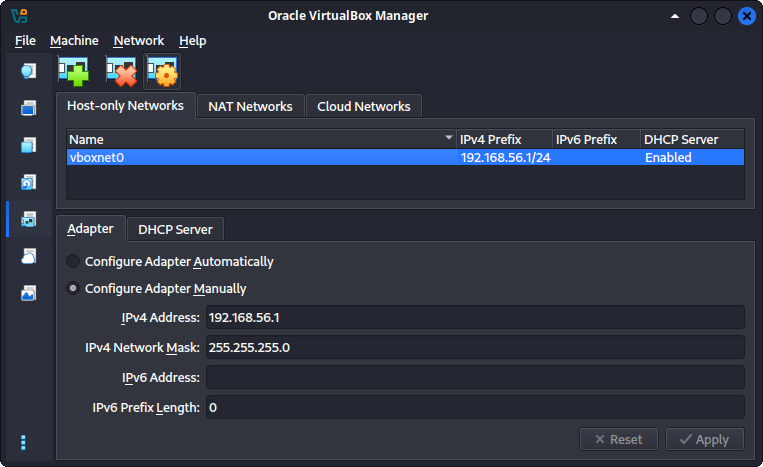
\includegraphics[width=0.48\textwidth]{images/net_setup_1.png}
        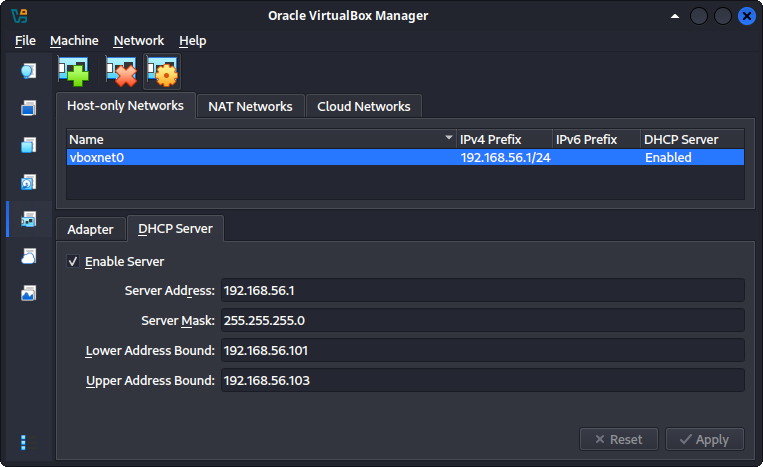
\includegraphics[width=0.48\textwidth]{images/net_setup_2.png}
    \end{center}
    \begin{enumerate}
        \item Go to Networks Settings and create a new Host-only Network
        \item Enable DHCP server and set the IP range enough to accommodate 3 VMs
        \item Save the configuration and remember the name of the network
    \end{enumerate}
\end{frame}

\begin{frame}
    \frametitle{Configure VM Network Settings}
    \begin{columns}[T,onlytextwidth]
        \begin{column}{0.4\textwidth}
            These are the 3 VMs:
            \begin{itemize}
                \item OPENVAS-FREE-24.10.9-VirtualBox
                \item Debian
                \item Windows XP
            \end{itemize}
            Configure the Network \underline{of all of them}
            by selecting the \textbf{Host-only Adapter} as network adapter 
            and choosing the network you created in the previous step.
        \end{column}
        \begin{column}{0.6\textwidth}
            \centering
            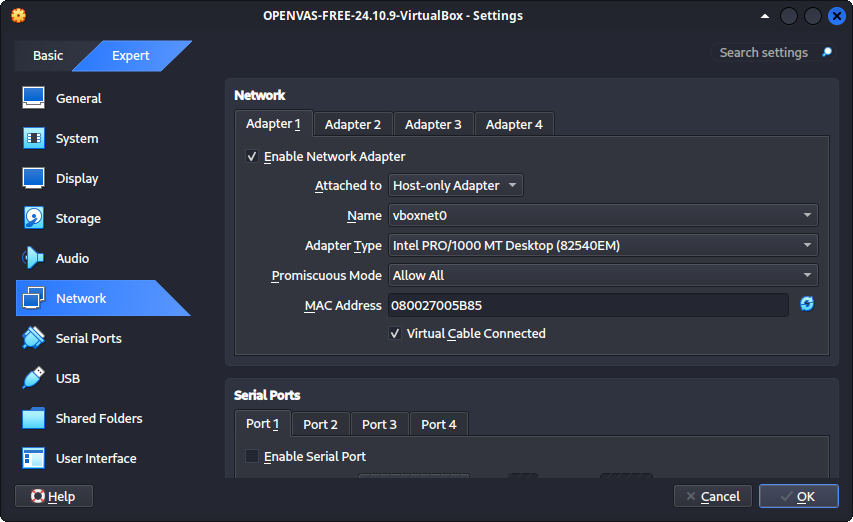
\includegraphics[width=\textwidth]{images/net_setup_3.png}
        \end{column}
    \end{columns}
\end{frame}

\begin{frame}[fragile]
    \frametitle{Start VMs without GUI}
    \begin{center}
        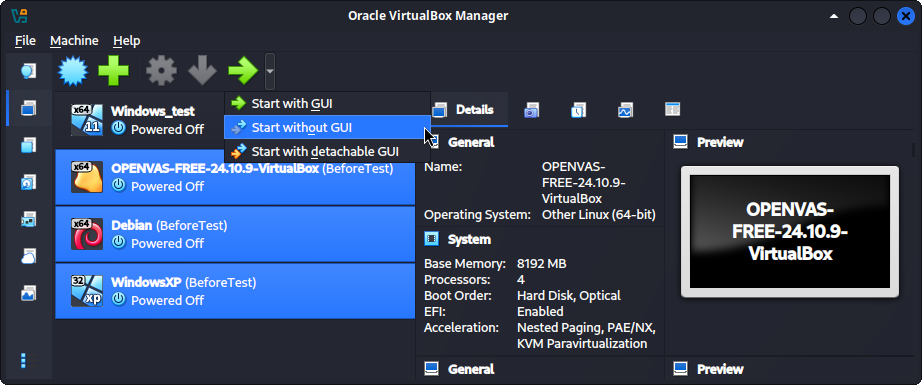
\includegraphics[width=0.8\textwidth]{images/vb-startup.png}
    \end{center}
    In order to save as much resources as possible, we will start the VMs without GUI.
    And since it will take a while to start, we will start them now and let them run in the background while we talk about the theory.
\end{frame}

\section{Vulnerability Assessment}

\sectionframe	% section title is automatically capitalised

\begin{frame}[fragile]
\frametitle{Vulnerability Assessment Process}
% place the small image to the left and scale to fit within the frame
\begin{center}
    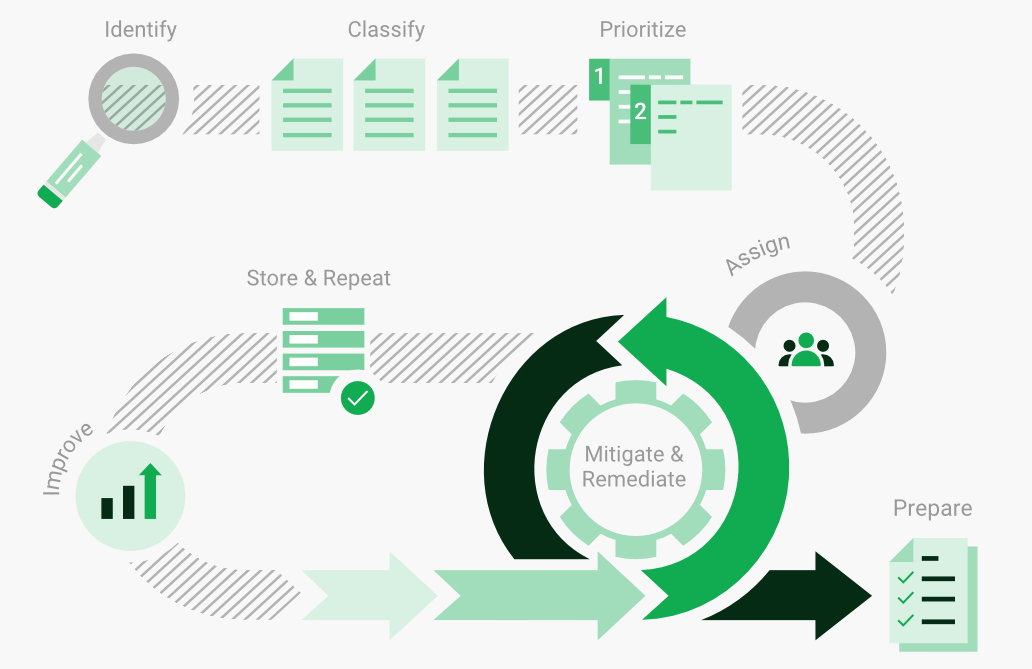
\includegraphics[width=0.8\textwidth]{images/greenbone_graph_2.jpg}
\end{center}

\end{frame}

\begin{frame}[fragile]
\frametitle{Vulnerability Scanning}
\begin{center}
\begin{minipage}{0.35\textwidth}
\centering
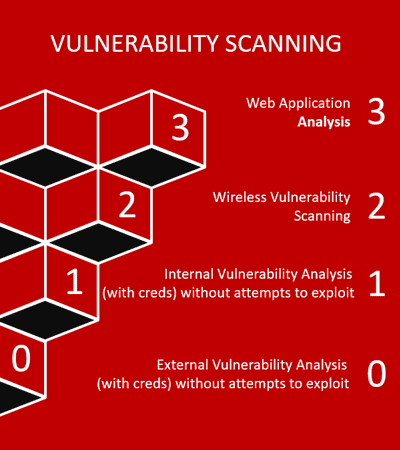
\includegraphics[width=\linewidth]{images/va_red.png}
\end{minipage}\hfill
\begin{minipage}{0.55\textwidth}
\centering
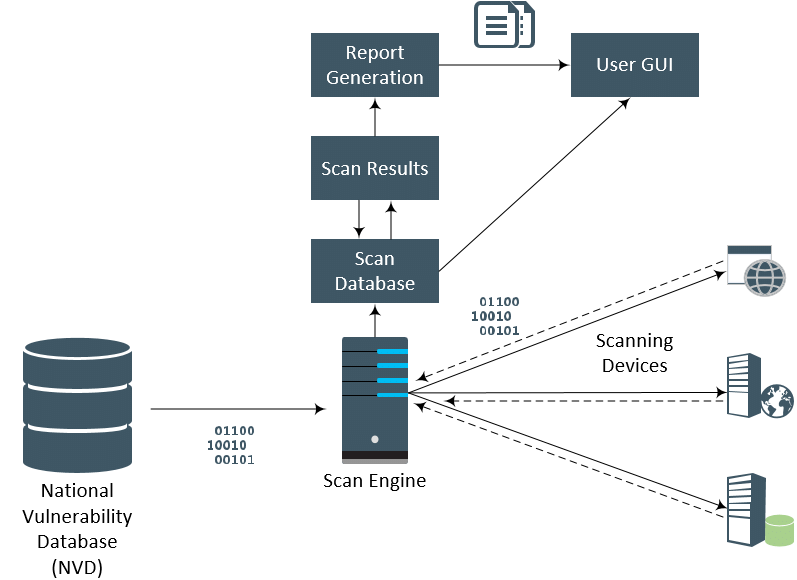
\includegraphics[width=\linewidth]{images/scan_engine_diagram.png}
\end{minipage}
\end{center}
\end{frame}

\section{OpenVAS}
\sectionframe

\begin{frame}[fragile]
\frametitle{Open Vulnerability Assessment Scanner (OpenVAS) by Greenbone}
	\begin{center}
		
\includegraphics[width=0.45\textwidth]{images/greenbone_logo.png}
		\href{https://github.com/greenbone/openvas-scanner}{https://github.com/greenbone/openvas-scanner}
	\end{center}
\end{frame}

\begin{frame}[fragile]
\frametitle{OpenVAS Architecture}
	\begin{center}
		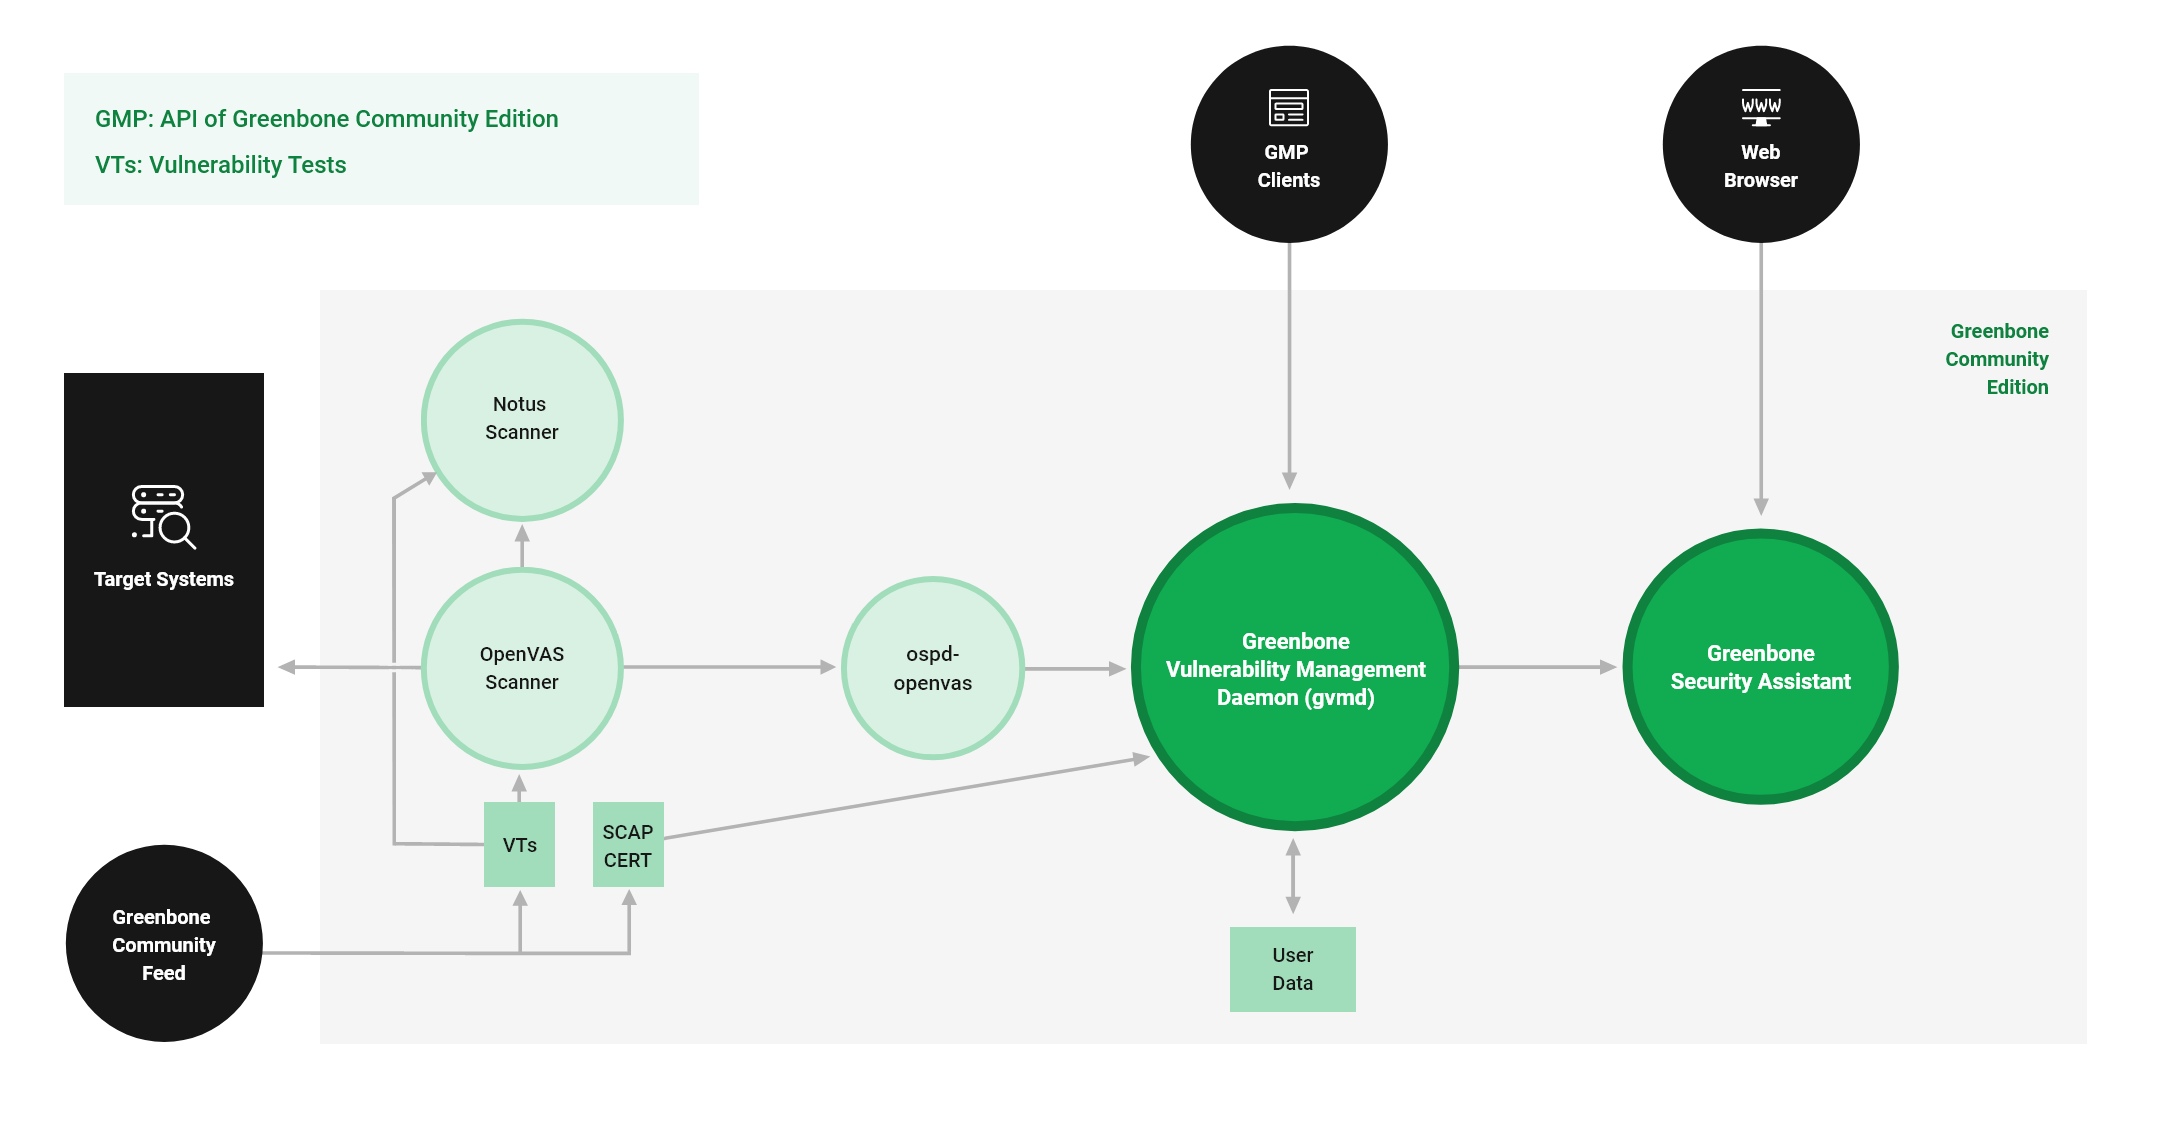
\includegraphics[width=1.0\textwidth]{images/openvas_architecture.png}
	\end{center}
\end{frame}

\section{Vulnerability Database}
\sectionframe

\begin{frame}[fragile]
\frametitle{Greenbone Database}
\begin{columns}[T,totalwidth=\textwidth]
\begin{column}{0.75\textwidth}
The Database is the core of OpenVAS.\\
It contains all the information about the vulnerabilities
and the way to check them.\\
\begin{tabular}{|c|c|}
    \hline
    \textbf{Type of Feed} & \textbf{Price} \\
    \hline
    Greenbone Community Feed & Free \\
    \hline
    Greenbone Security Feed & 2524 €/year \\
    \hline
\end{tabular}


\includegraphics[width=0.75\textwidth]{images/GSF.png}
\end{column}
\begin{column}{0.25\textwidth}

\begin{figure}
\begin{center}

\includegraphics[height=0.4\textheight]{images/postgesql.png}
\end{center}
\end{figure}
\end{column}
\end{columns}
\end{frame}

\begin{frame}[fragile]
    \frametitle{Database's Structure}
    \begin{columns}[T,totalwidth=\textwidth]
    \begin{column}{0.33\textwidth}
        \begin{center}
        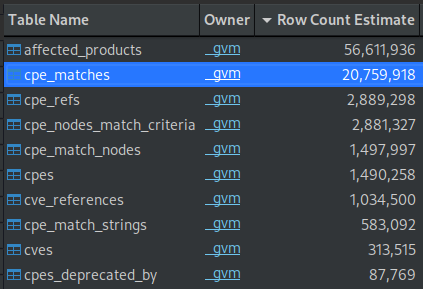
\includegraphics[width=0.95\textwidth]{images/db1.png}\\[50pt]
        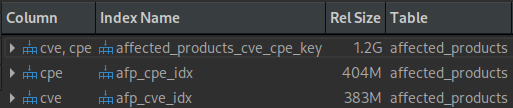
\includegraphics[width=0.95\textwidth]{images/db3.png}
        \end{center}
    \end{column}
    \begin{column}{0.34\textwidth}
        %\begin{center}
        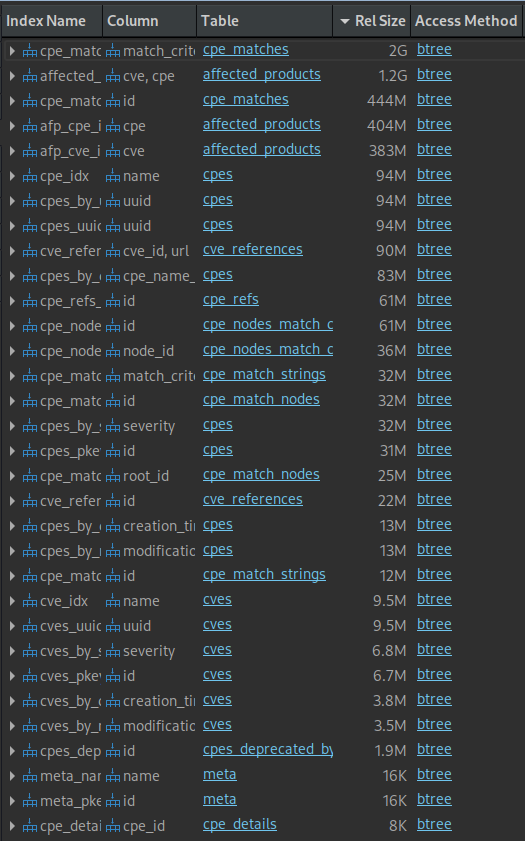
\includegraphics[width=1.0\textwidth]{images/db5.png}
        %\end{center}
    \end{column}
    \begin{column}{0.33\textwidth}
        \begin{center}
        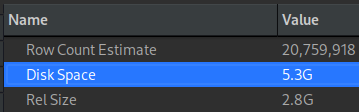
\includegraphics[width=0.95\textwidth]{images/db4.png}\\[70pt]
        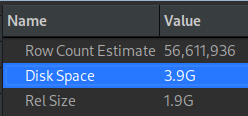
\includegraphics[width=0.95\textwidth]{images/db2.png}
        \end{center}
    \end{column}
    \end{columns}
\end{frame}

\begin{frame}[fragile]
    \frametitle{Feed Update}
    \begin{columns}[T,totalwidth=\textwidth]
    \begin{column}{0.5\textwidth}
    %    \begin{center}
        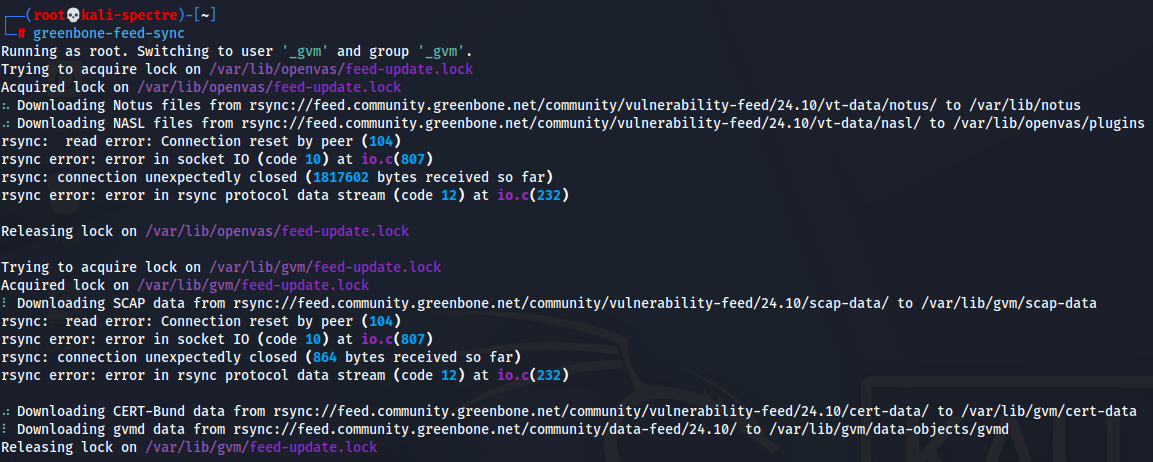
\includegraphics[width=0.95\textwidth]{images/screen_gvm1.png}\\
        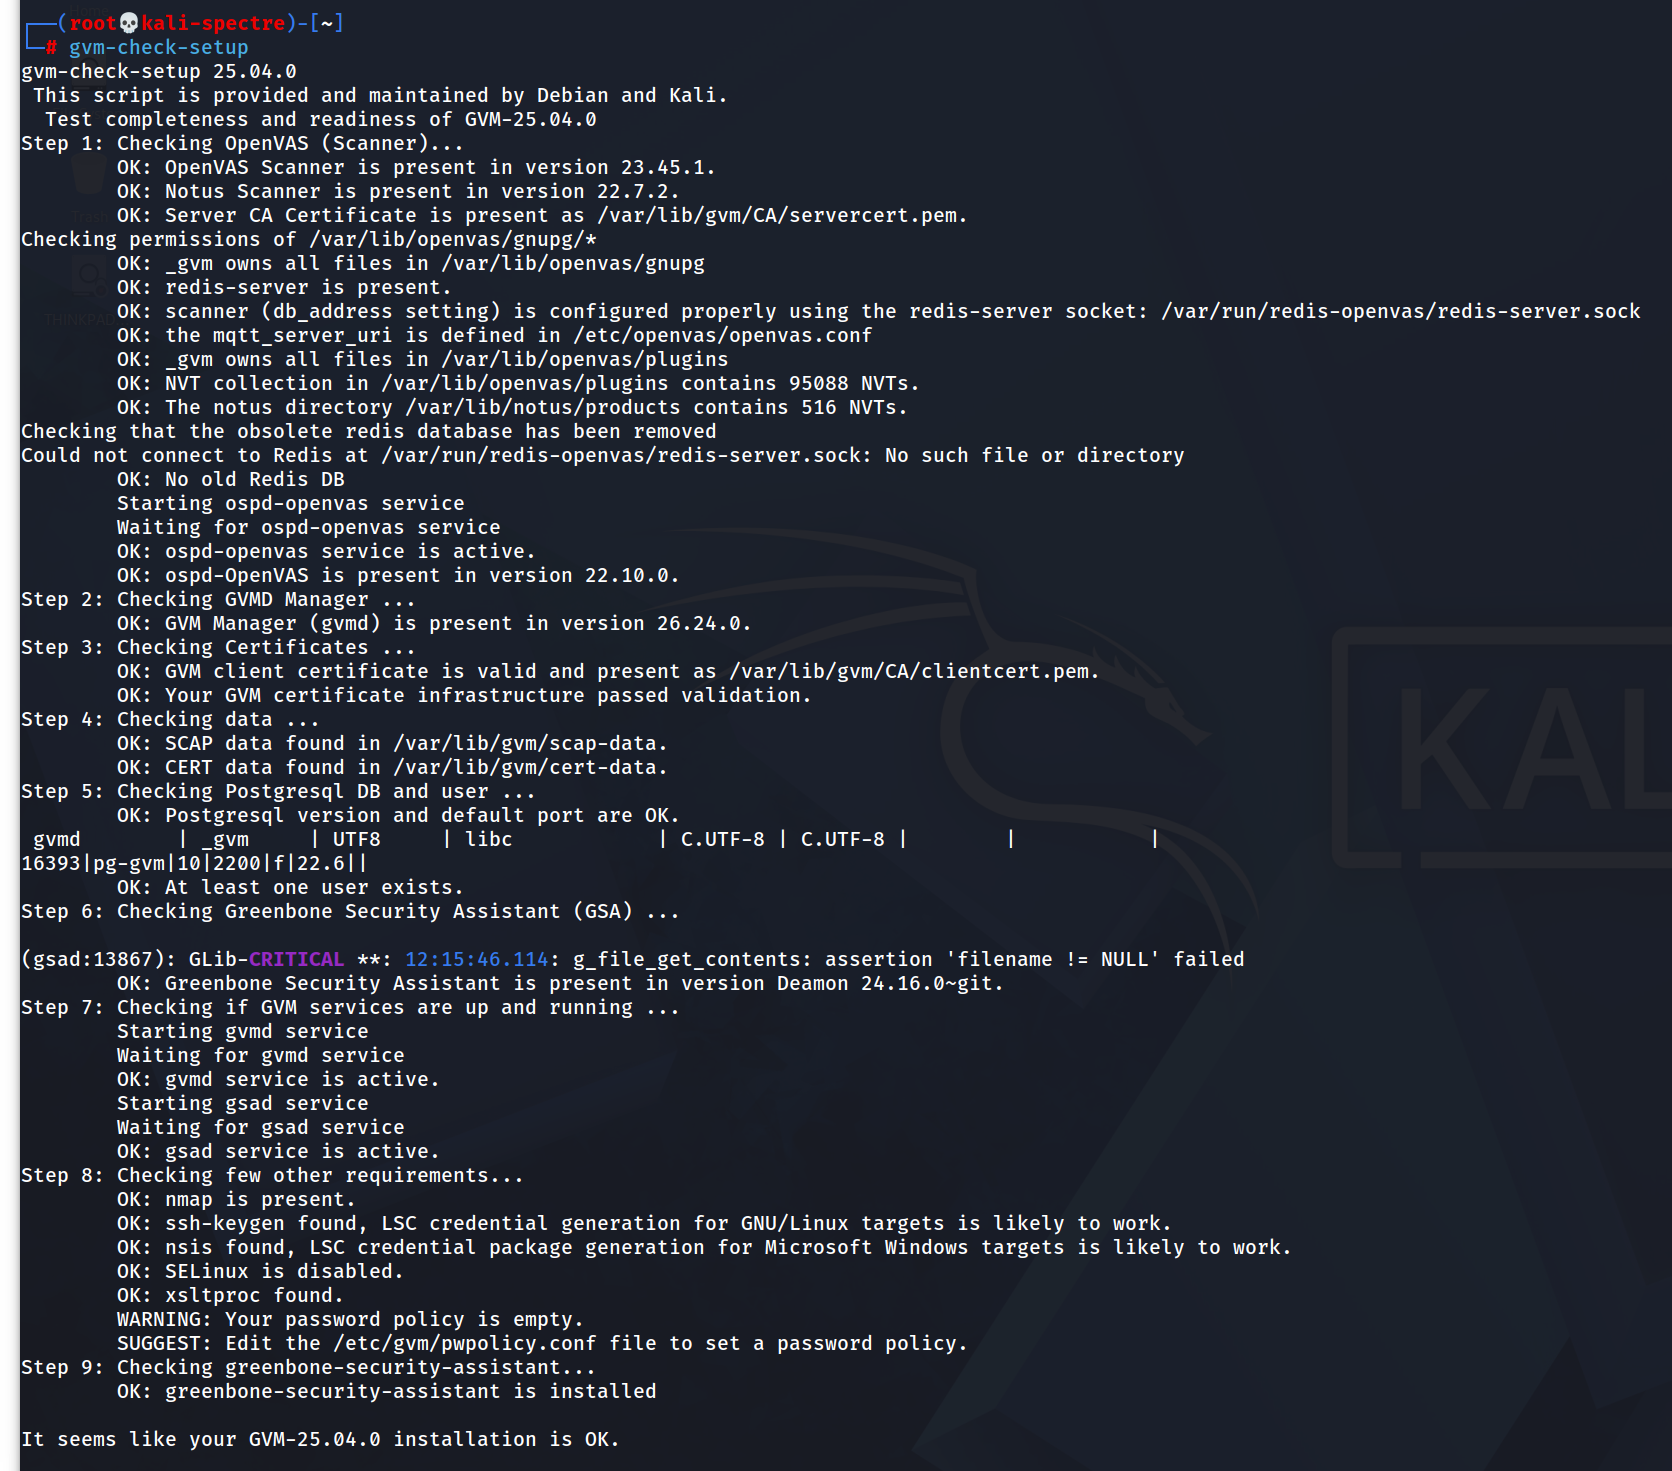
\includegraphics[width=0.7\textwidth]{images/screen_gvm2.png}
    %    \end{center}
    \end{column}
    \begin{column}{0.5\textwidth}
    %    \begin{center}
        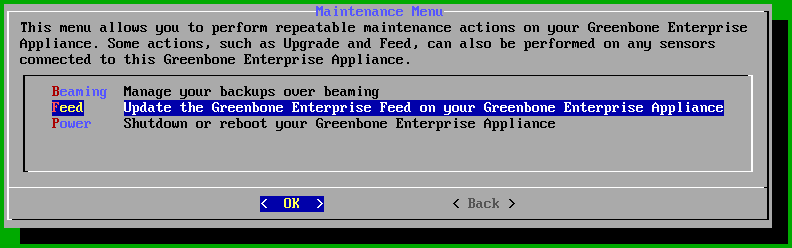
\includegraphics[width=0.9\textwidth]{images/gs_feed_update.png}\\[4pt]
        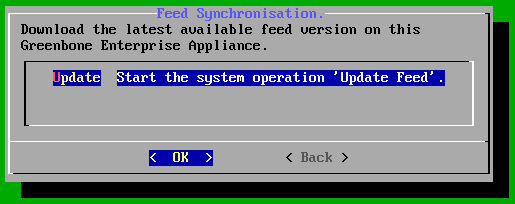
\includegraphics[width=0.9\textwidth]{images/gs_feed_update2.png}\\[4pt]
        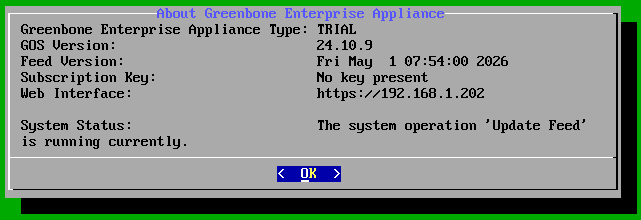
\includegraphics[width=0.9\textwidth]{images/gs_info.png}
    %    \end{center}
    \end{column}    
    \end{columns}
\end{frame}

\begin{frame}[fragile]
    \frametitle{Feed Status}
    \begin{center}
        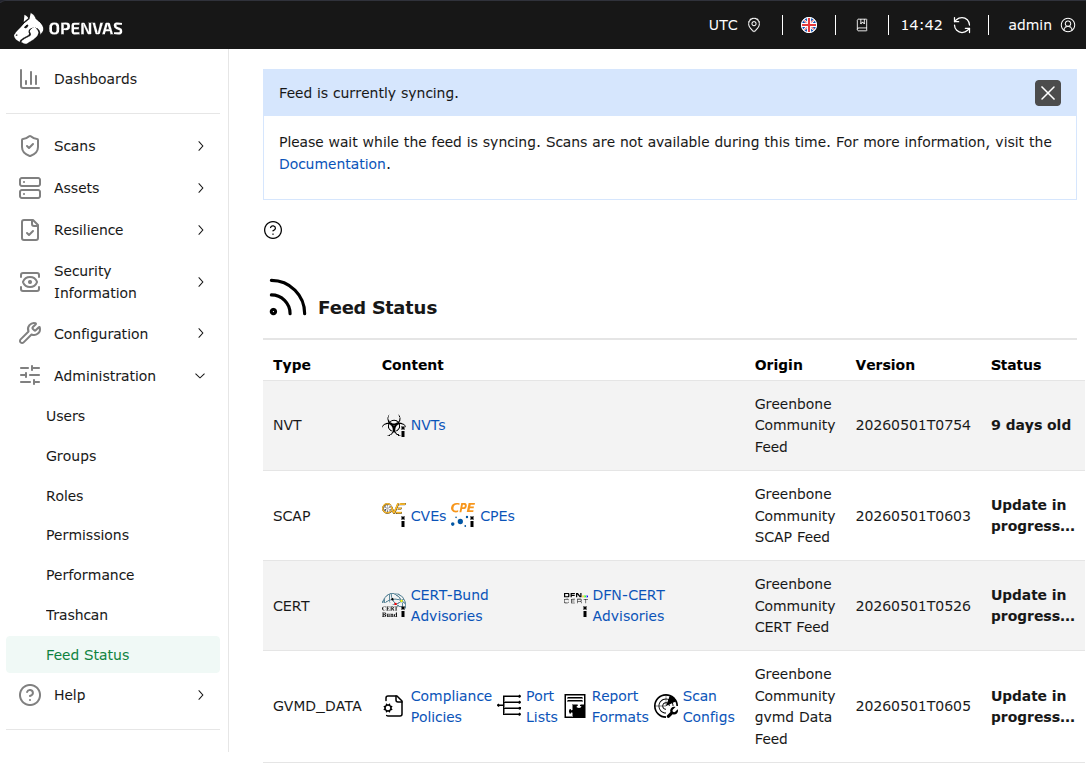
\includegraphics[height=0.75\textheight]{images/gs_feed_status.png}
    \end{center}
\end{frame}

\section{System Overview}
\sectionframe

\begin{frame}[fragile]
    \frametitle{Network}
    \begin{center}
        \ifdarktheme
            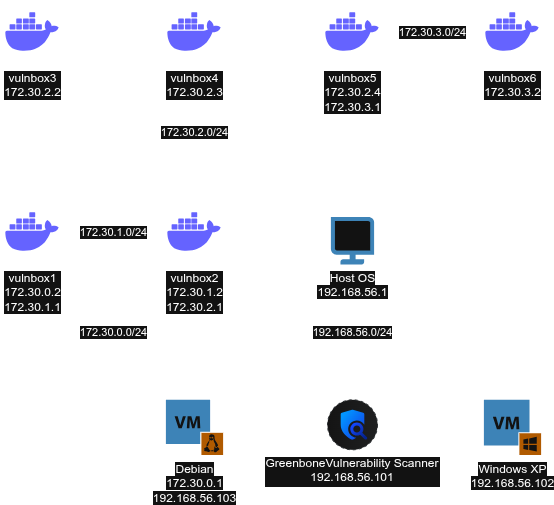
\includegraphics[width=0.55\textwidth]{images/net-sec-lab.png}
        \else
            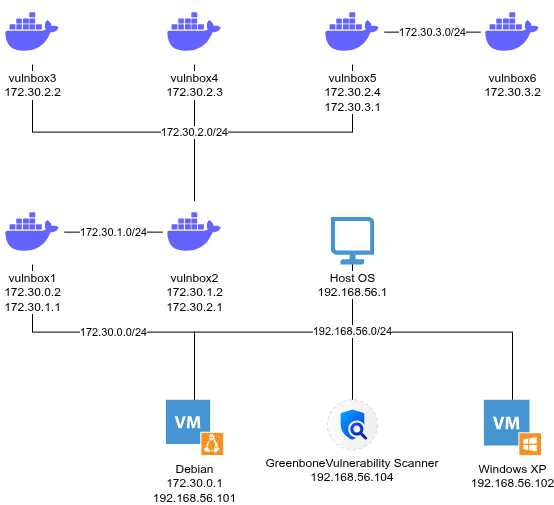
\includegraphics[width=0.55\textwidth]{../project/net-sec-lab.png}
        \fi
    \end{center}
\end{frame}

\section{Setup Greenbone}
\sectionframe
\begin{frame}
    \frametitle{Debian}
    \begin{columns}
        \begin{column}{0.25\textwidth}
            \begin{itemize}
                \item Show the Debian VM
                \item Go to the VM's console
                \item Log in with the credentials \texttt{root:root}
            \end{itemize}
        \end{column}
        \begin{column}{0.75\textwidth}
            \begin{center}
                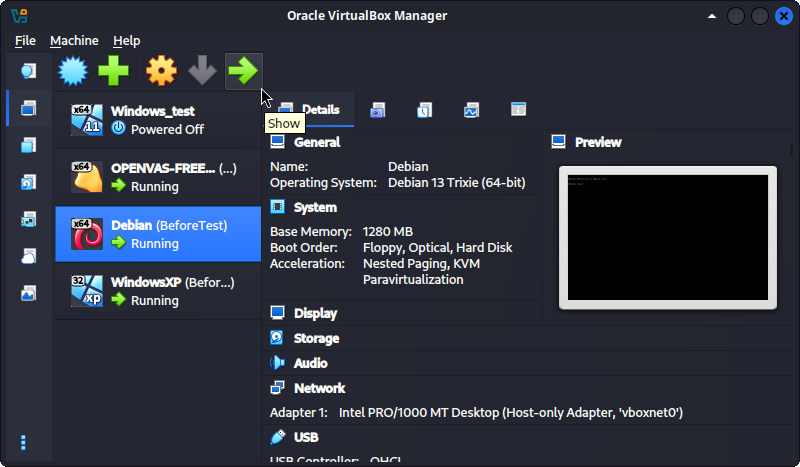
\includegraphics[width=1.0\textwidth]{images/debian_show.png}
            \end{center}
        \end{column}
    \end{columns}
\end{frame}

\begin{frame}
    \frametitle{Launch a bash script in Debian}
    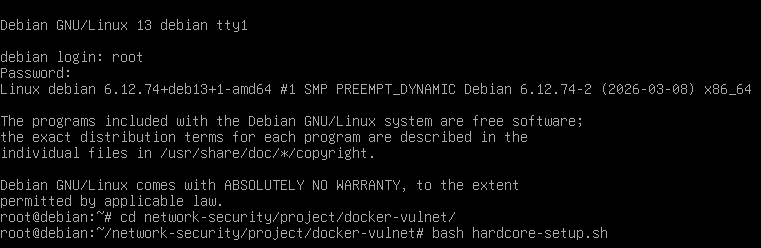
\includegraphics[width=1.0\textwidth]{images/debian_start.png}
    \texttt{cd network-security/project/docker-vulnet/}\\
    \texttt{bash hardcore-setup.sh}
\end{frame}

\begin{frame}[fragile]
    \frametitle{Check Debian IP Address}
    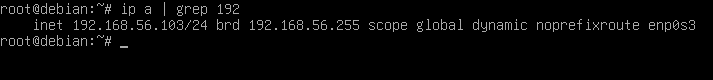
\includegraphics[width=1.0\textwidth]{images/debian_ip.png}
    \texttt{ip a | grep 192}\\
    It should output something like \texttt{192.160.56.10X}
\end{frame}

\begin{frame}[fragile]
    \frametitle{Set Greenbone Gateway}
    \begin{center}
        \begin{tabular}{cc}
            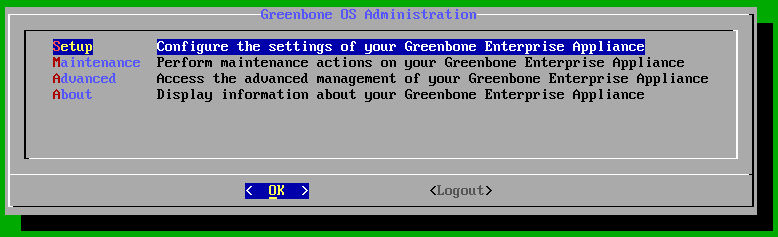
\includegraphics[width=0.47\textwidth]{images/gs_gateway_1.png} &
            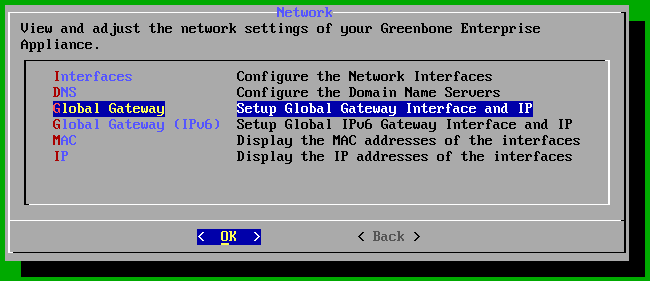
\includegraphics[width=0.47\textwidth]{images/gs_gateway_3.png} \\
            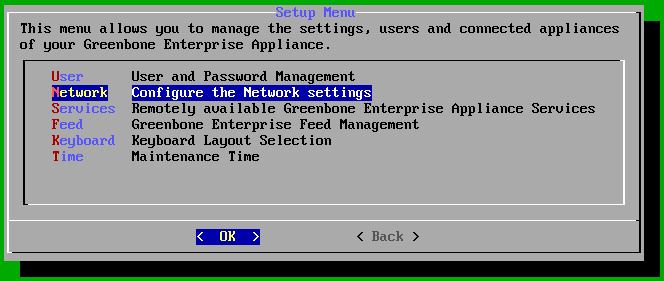
\includegraphics[width=0.47\textwidth]{images/gs_gateway_2.png} &
            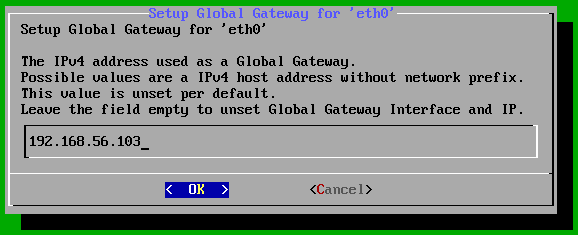
\includegraphics[width=0.47\textwidth]{images/gs_gateway_4.png}
        \end{tabular}
    \end{center}
\end{frame}

\begin{frame}[fragile]
    \frametitle{Remeber to save the settings}
    \begin{center}
        \begin{tabular}{cc}
            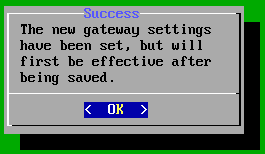
\includegraphics[height=0.375\textheight]{images/gs_gateway_5.png} &
            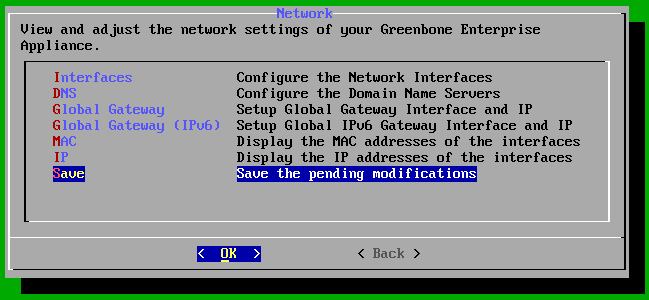
\includegraphics[height=0.375\textheight]{images/gs_gateway_6.png}
        \end{tabular}
    \end{center}
\end{frame}

\section{System Discovery}
\sectionframe

\begin{frame}[fragile]
    \frametitle{Open the Greenbone Web Interface}
    \begin{columns}
        \begin{column}{0.6\textwidth}
            \begin{itemize}
                \item Check your Greenbone's IP address in 
                the \textbf{About} option
                \item Open a web browser
                \item Go to \texttt{https://192.160.56.10X/}
                (Your Greenbone's IP address)
                \item Log in with the credentials \texttt{admin:admin}
            \end{itemize}
        \end{column}
        \begin{column}{0.4\textwidth}
            \begin{center}
                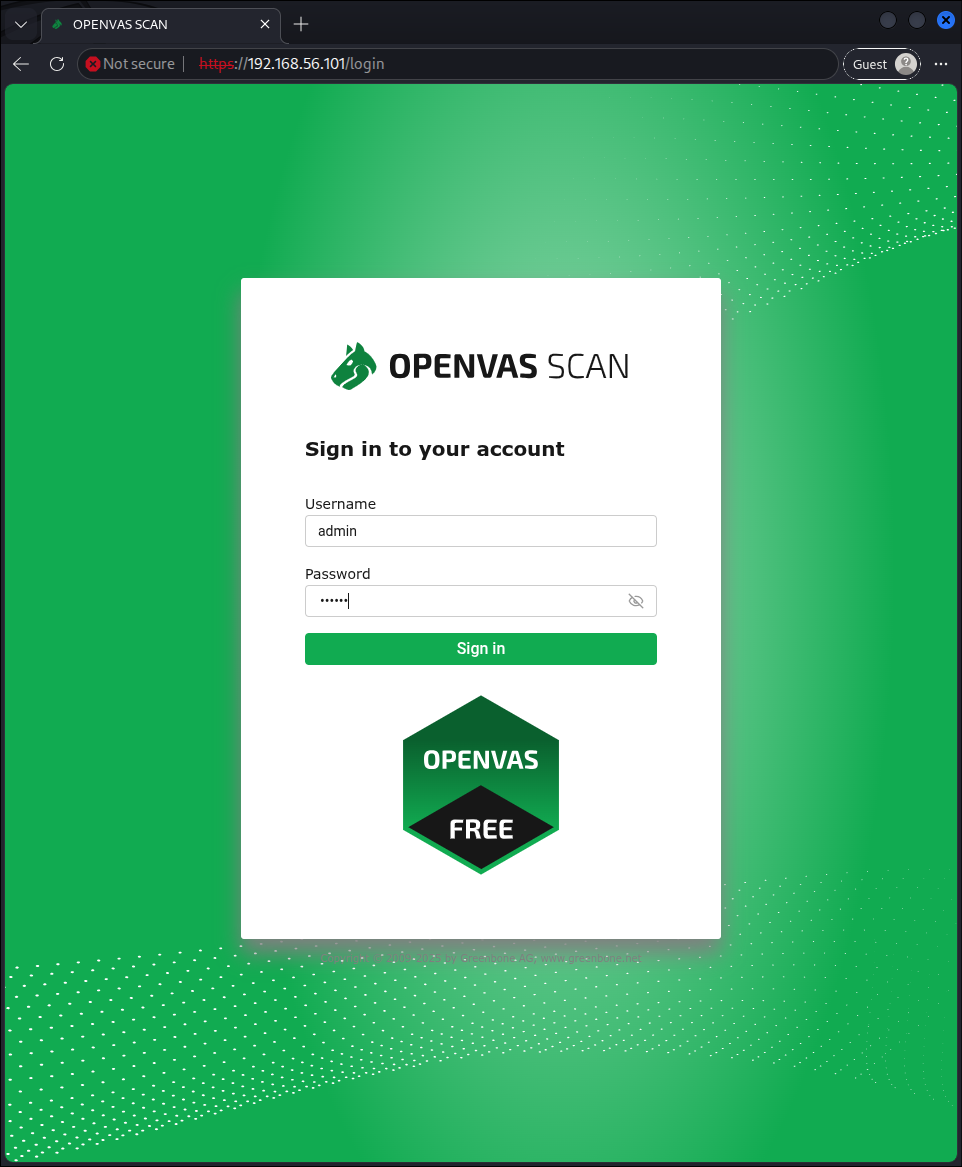
\includegraphics[width=1.0\textwidth]{images/gs_web_login.png}
            \end{center}
        \end{column}
    \end{columns}
\end{frame}

\begin{frame}[fragile]
    \frametitle{Network Scan}
    \begin{center}
        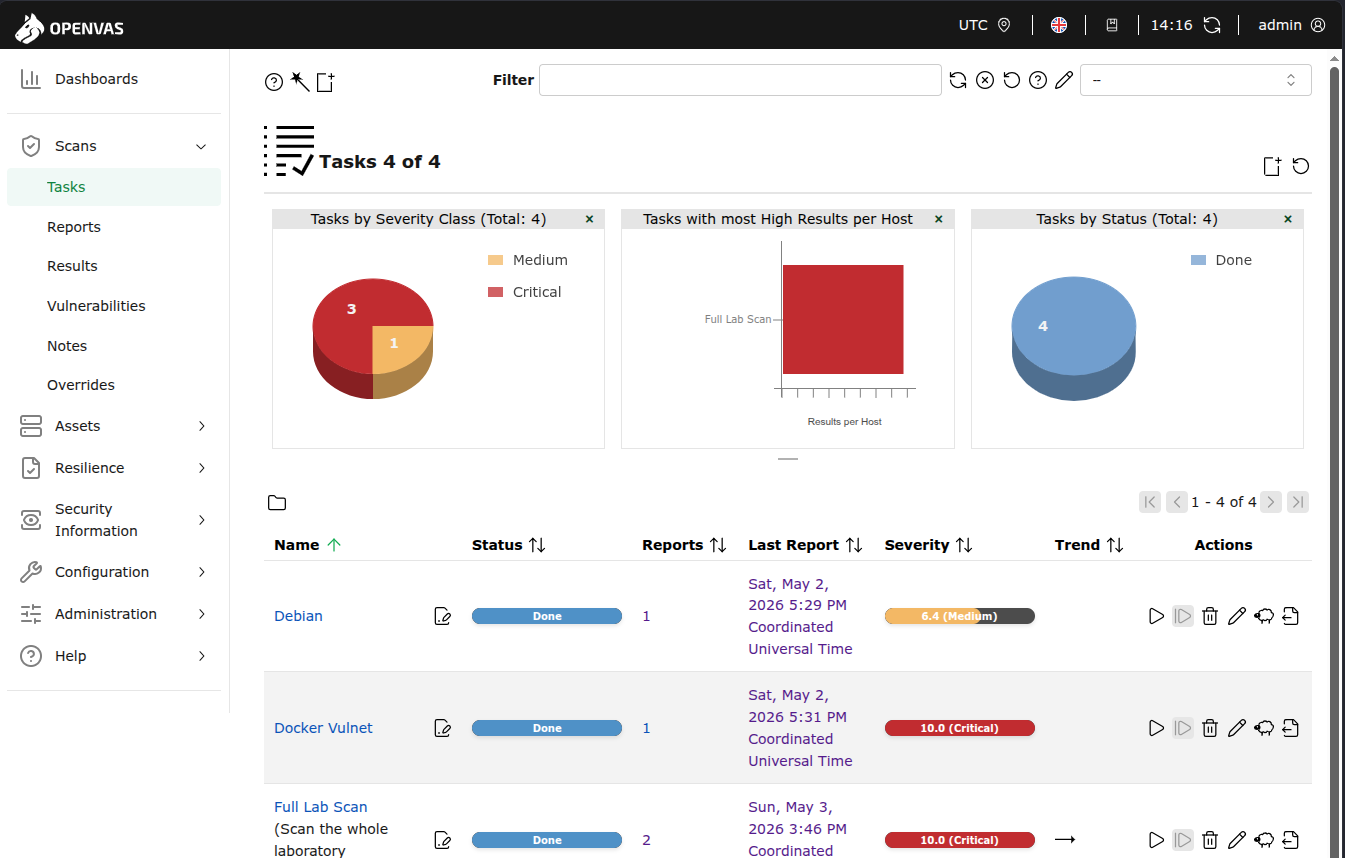
\includegraphics[width=0.8\textwidth]{images/gs_sd_1.png}
    \end{center}
\end{frame}

\begin{frame}[fragile]
    \frametitle{Configuration of the Scan}
    \begin{center}
        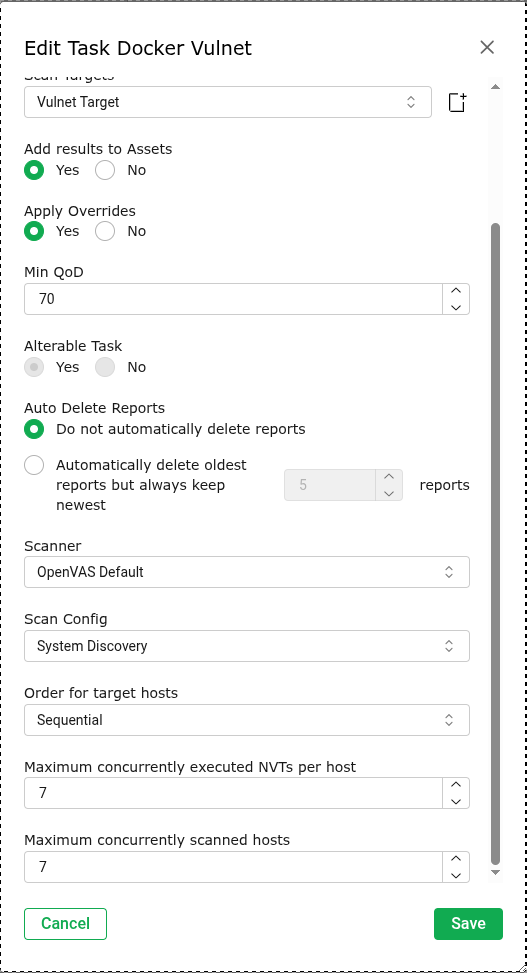
\includegraphics[height=0.8\textheight]{images/gs_sd_2.png}
    \end{center}
\end{frame}

\begin{frame}[fragile]
    \frametitle{Start the Scan}
    \begin{center}
        
\includegraphics[width=1.0\textwidth]{images/gs_sd_3.png}\\[10pt]
        
\includegraphics[width=1.0\textwidth]{images/gs_sd_5.png}
    \end{center}
\end{frame}

\begin{frame}[fragile]
    \frametitle{Scan Results}
    \begin{center}
        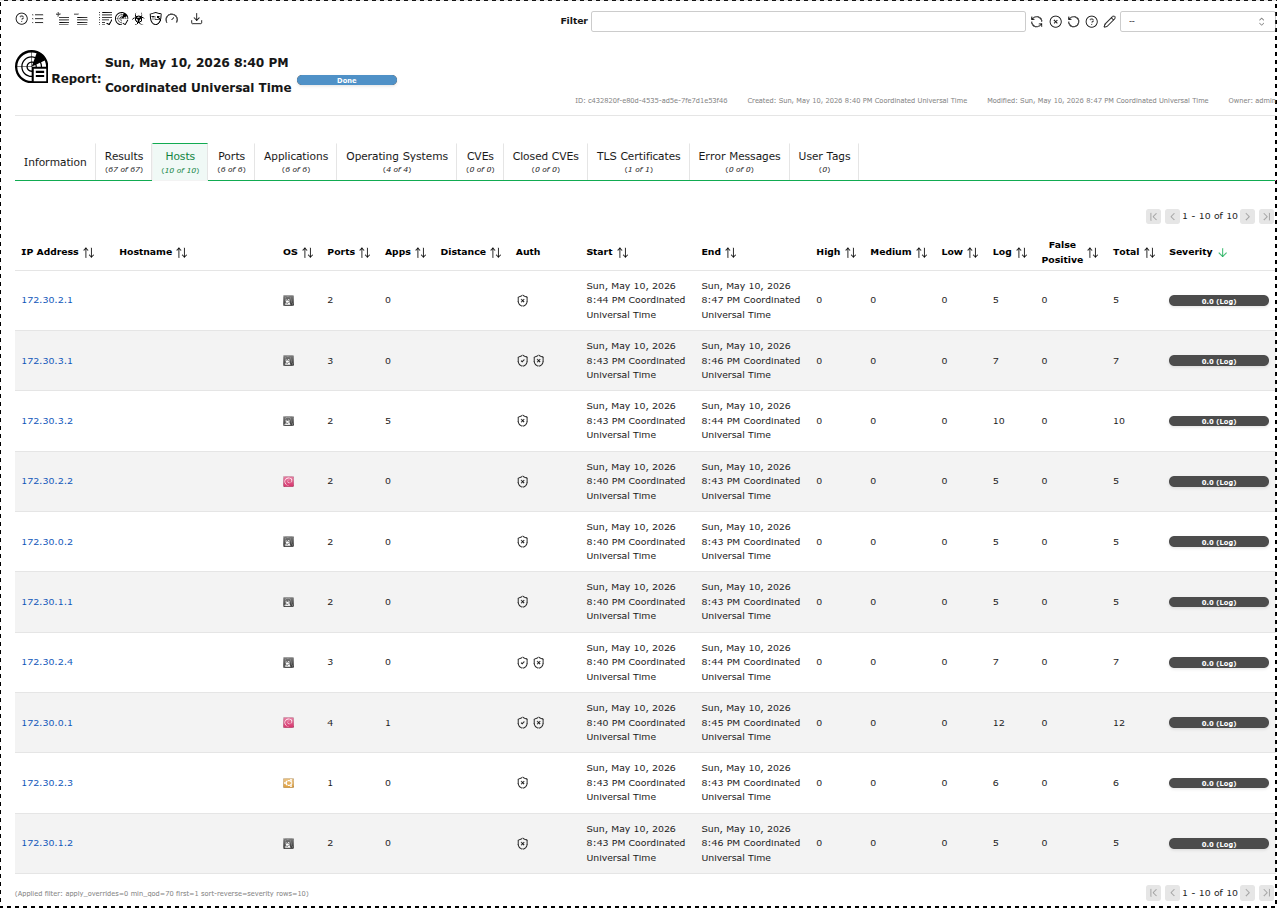
\includegraphics[width=1.0\textwidth]{images/gs_sd_6.png}
    \end{center}
\end{frame}

\section{Vulnerability scan}

\sectionframe

\frame{
	\frametitle{What we will do}

	\begin{columns}[T,onlytextwidth]
        \begin{column}{0.4\textwidth}
            We will:
            \begin{itemize}
                \item Explain VMs and vulnerable services
                \item Look at OpenVAS interface and tools
                \item Scan targets
				\item Look at a complete report
            \end{itemize}
        
		\end{column}
    \end{columns}
}


\frame{
	\frametitle{Debian VM}
	\begin{columns}[T,onlytextwidth]
        \begin{column}{0.4\textwidth}
            Vulnerable services
            \begin{itemize}
				\item Apache 
				\item CUPS
				\item FTP
				\item Samba
				\item SSH
				\item Syslog
            \end{itemize}
		\end{column}

		\begin{column}{0.5\textwidth}
            \centering
            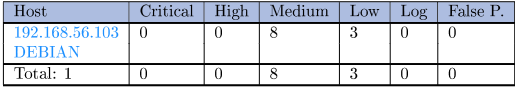
\includegraphics[width=\textwidth, height=0.4\textheight, keepaspectratio]{images/debian_vuln1.png}
            
            \vspace{0.5cm} % Adjust the gap between images here
            
            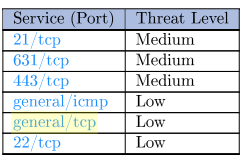
\includegraphics[width=\textwidth, height=0.3\textheight, keepaspectratio]{images/debian_vuln2.png}
        \end{column}

    \end{columns}
}

\frame{
	\frametitle{Windows XP}
	\begin{columns}[T,onlytextwidth]
        \begin{column}{0.4\textwidth}
            Vulnerable services
            \begin{itemize}
				\item FTP
				\item Firewall (inexsistent)
				\item General legacy things
            \end{itemize}
		\end{column}

		\begin{column}{0.5\textwidth}
            \centering
            \includegraphics[width=\textwidth, height=0.4\textheight, keepaspectratio]{images/Windows_vuln1.png}
            
            \vspace{0.5cm} % Adjust the gap between images here
            
            \includegraphics[width=\textwidth, height=0.3\textheight, keepaspectratio]{images/Windows_vuln2.png}
			\hfill
			\includegraphics[width=\textwidth, height=0.3\textheight, keepaspectratio]{images/Windows_vuln3.png}

        \end{column}
    \end{columns}
}

\frame{
	\frametitle{Excercise: Find out hosts IPs}
	Since we've configured a virtual network with DHCP IPs may vary, so you have to find them
	\begin{columns}[T,onlytextwidth]
        \begin{column}{0.4\textwidth}
            Vulnerable services
            \begin{itemize}
				\item On Windows: Open window from VirtualBox, open terminal and find IP via ipconfig /all
				\item On OpenVAS: Just see the IP on the top
            \end{itemize}
		\end{column}

		\begin{column}{0.5\textwidth}
            \centering
            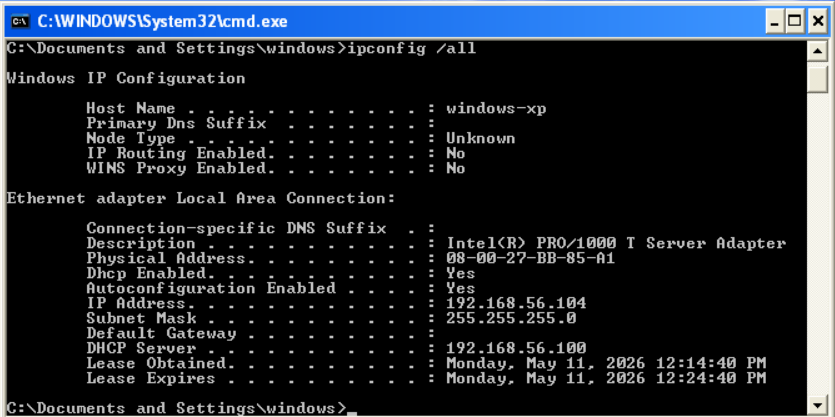
\includegraphics[width=\textwidth, height=0.4\textheight, keepaspectratio]{images/windowsxp_ipshow.png}

        \end{column}
    \end{columns}
}


\section{OpenVAS Interface}

\sectionframe


% \frame{
% 	\frametitle{The most important thing\: The Feed}
% 		\begin{columns}[T,onlytextwidth,c]
%         \begin{column}{0.3\textwidth}
% 			\begin{itemize}
% 				\item This is the most important aspect of the tool: without it nothing will work
% 				\item Will take a lot of time to sync
% 				\item Every startup it tries to sync
% 			\end{itemize}
% 		\end{column}
% 		\begin{column}{0.6\textwidth} % Give the column a width here
% 			\centering
% 			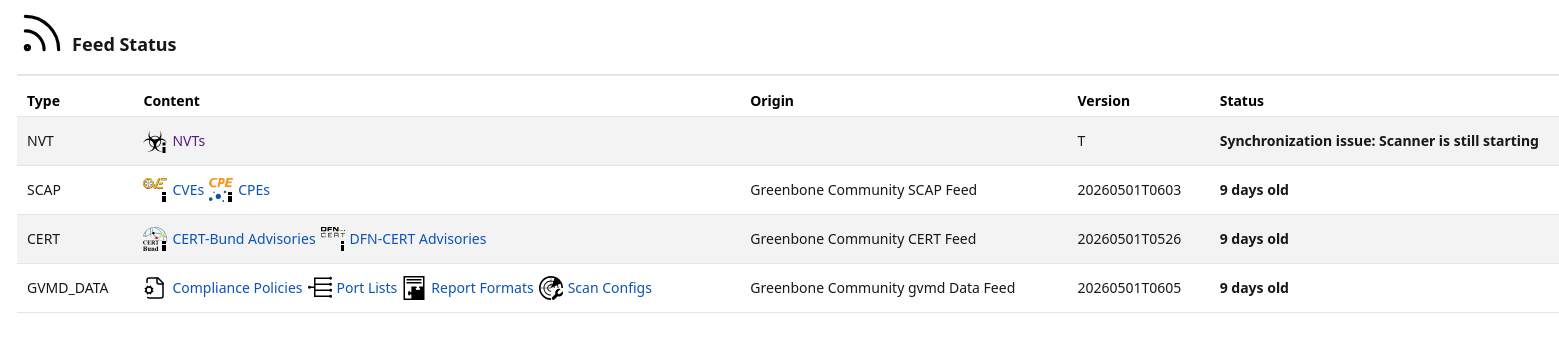
\includegraphics[width=\textwidth]{images/openvas_feed.png}
% 		\end{column}
%     \end{columns}
% }

\frame{
	\frametitle{Ports interface}
	\begin{center}
		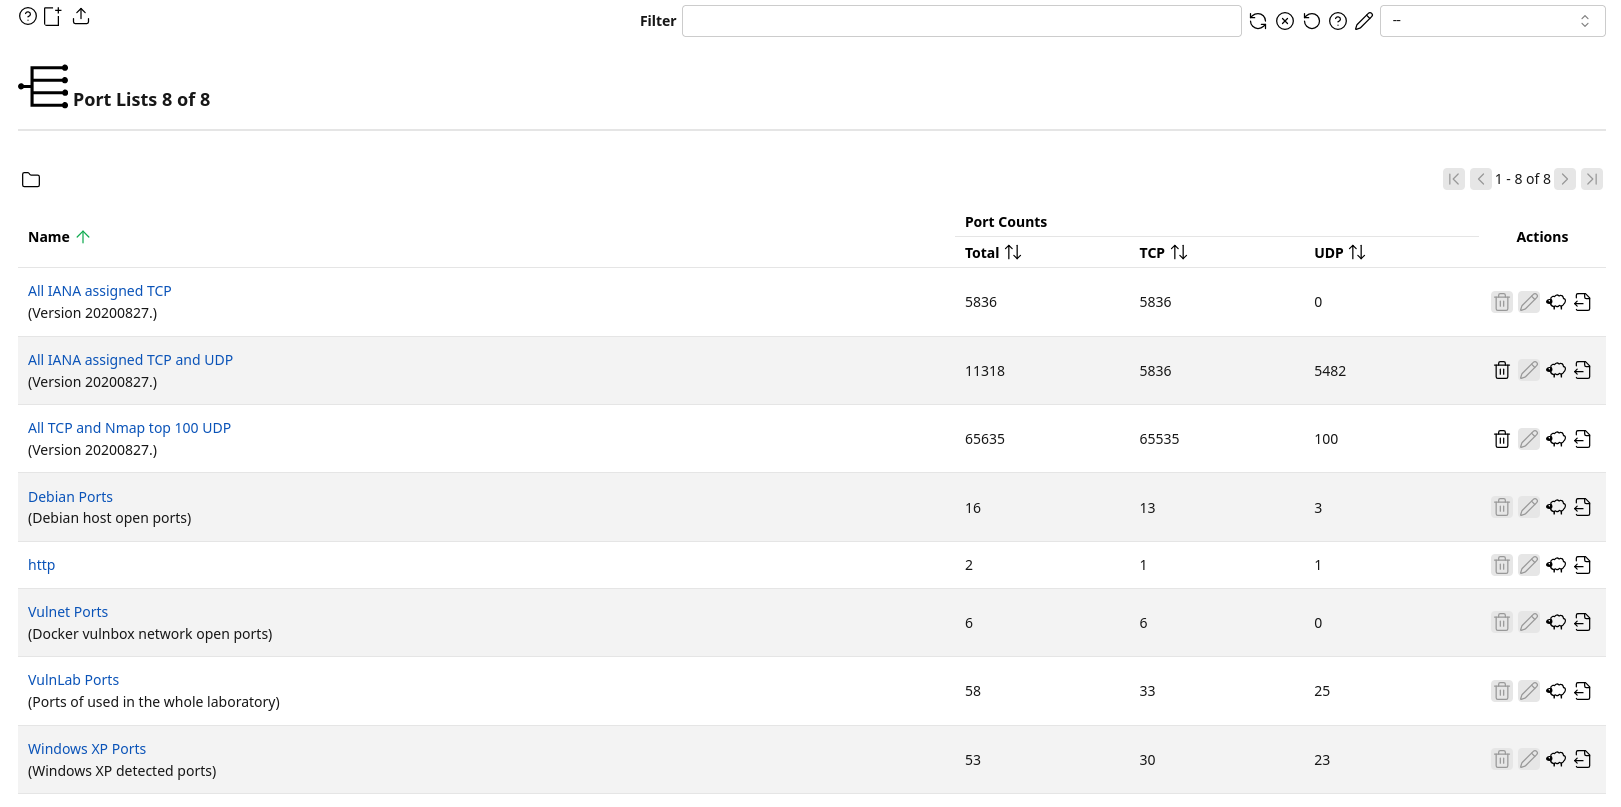
\includegraphics[width=0.9\textwidth]{images/openvas_ports_interface1.png}
	\end{center}

}

\frame{
	\frametitle{Port creation}
	\begin{columns}[T,onlytextwidth]
		\begin{column}{0.4\textwidth}
		\begin{itemize}
			\item Ports are expressed in its own format
			\item e.g. T:1-1024, 4500, U:1-100, 1023
		\end{itemize}
		\end{column}

       \begin{column}{0.6\textwidth}
           \centering
           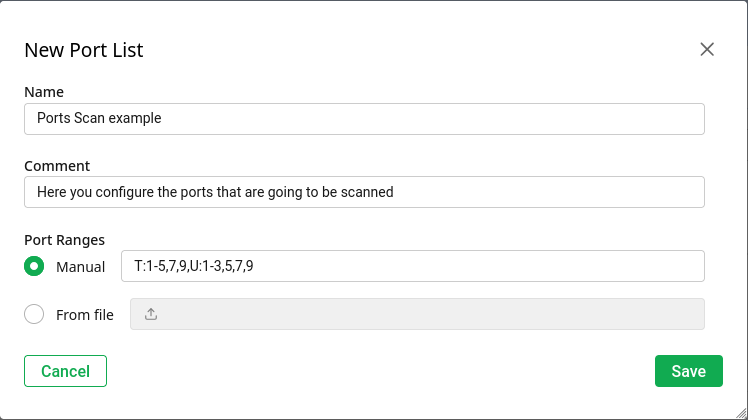
\includegraphics[width=\textwidth]{images/openvas_ports_scan1.png}
       \end{column}
    \end{columns}
}


\frame{
	\frametitle{Credentials for target access}
	\begin{columns}[T,onlytextwidth]
		\begin{column}{0.4\textwidth}
		\begin{itemize}
			\item You may also give the appliance the target credentials to have a more in-depth scan.
			\item It may improve accuracy since it scans more deeply, looking also at config files.
		\end{itemize}
		\end{column}

       \begin{column}{0.6\textwidth}
           \centering
           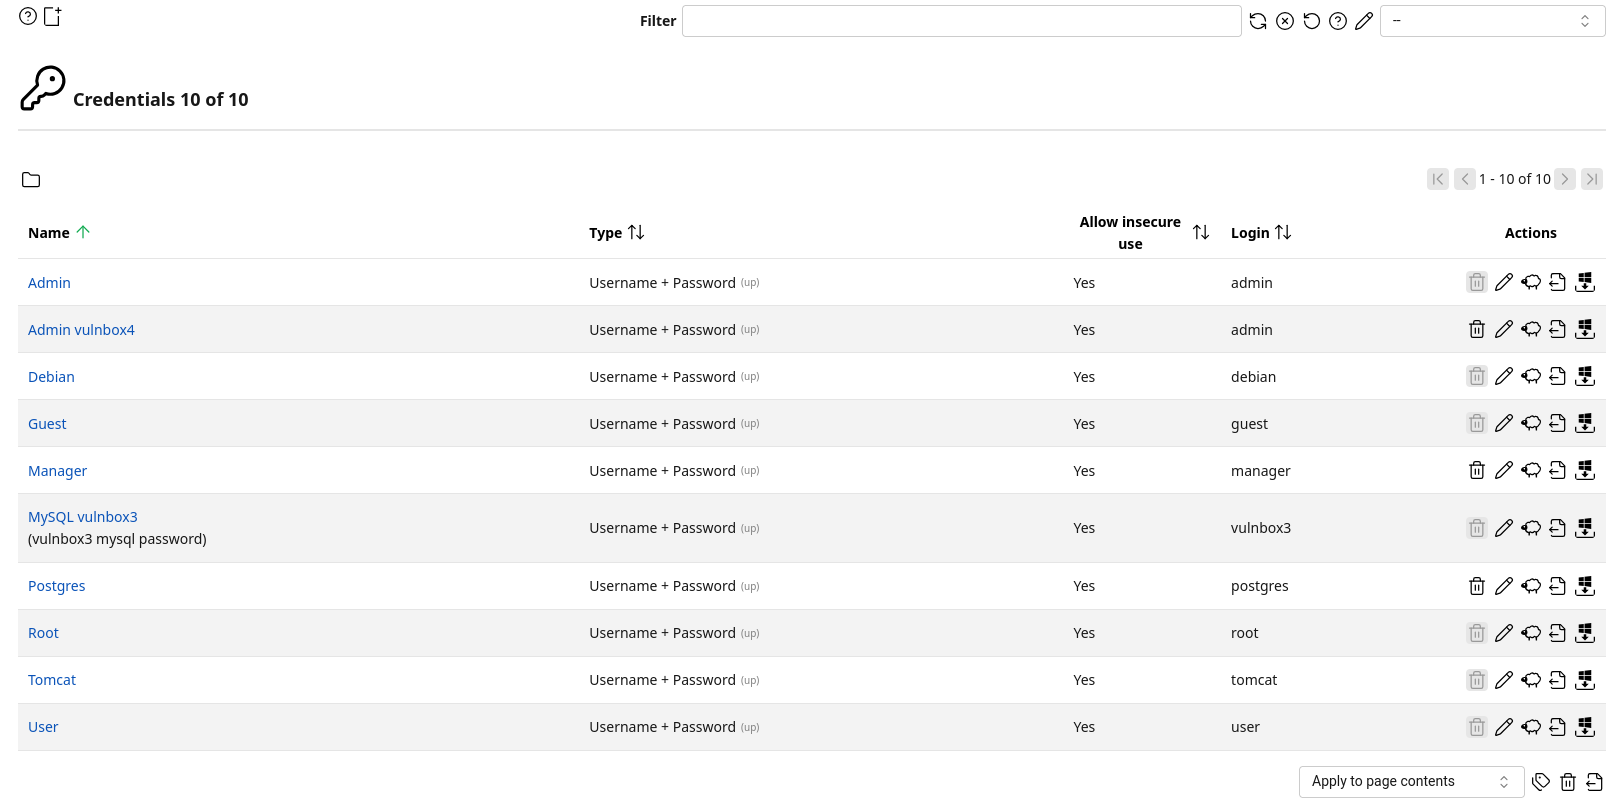
\includegraphics[width=\textwidth]{images/openvas_credentials1.png}
       \end{column}
    \end{columns}
}

\frame{
	\frametitle{Set scan credentials (for deeper scans)}
	\begin{columns}[T,onlytextwidth]
		\begin{column}{0.4\textwidth}
		   \centering
           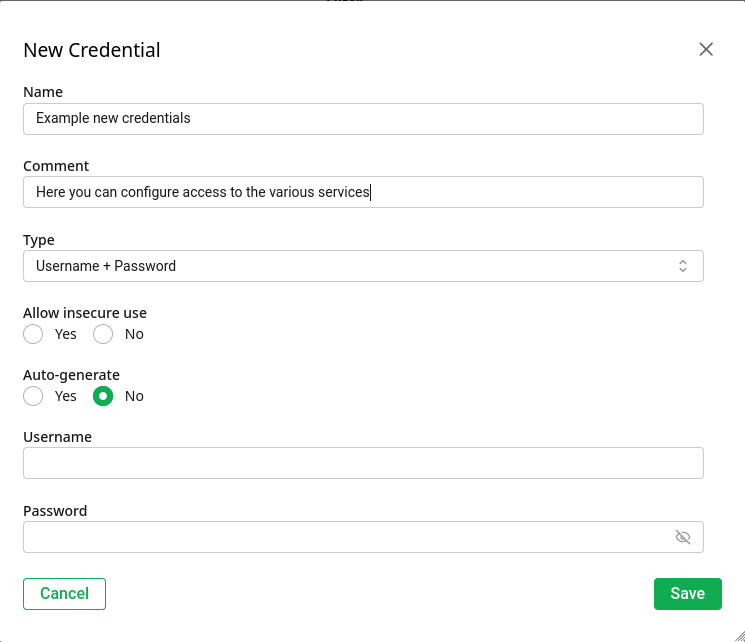
\includegraphics[width=\textwidth]{images/openvas_new_credentials1.png}
		\end{column}

       \begin{column}{0.4\textwidth}
           \centering
           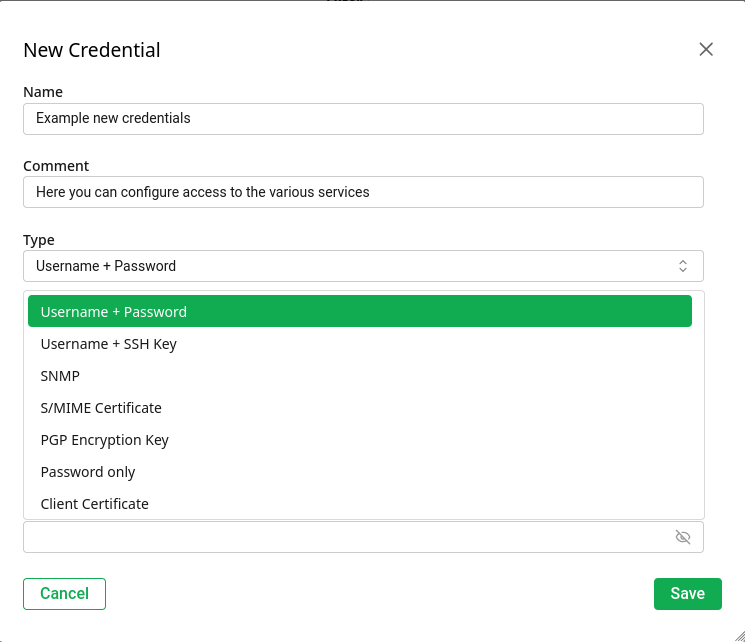
\includegraphics[width=\textwidth]{images/openvas_new_credentials2.png}
       \end{column}
    \end{columns}

}


\frame{
	\frametitle{Target interface}
	\begin{center}
		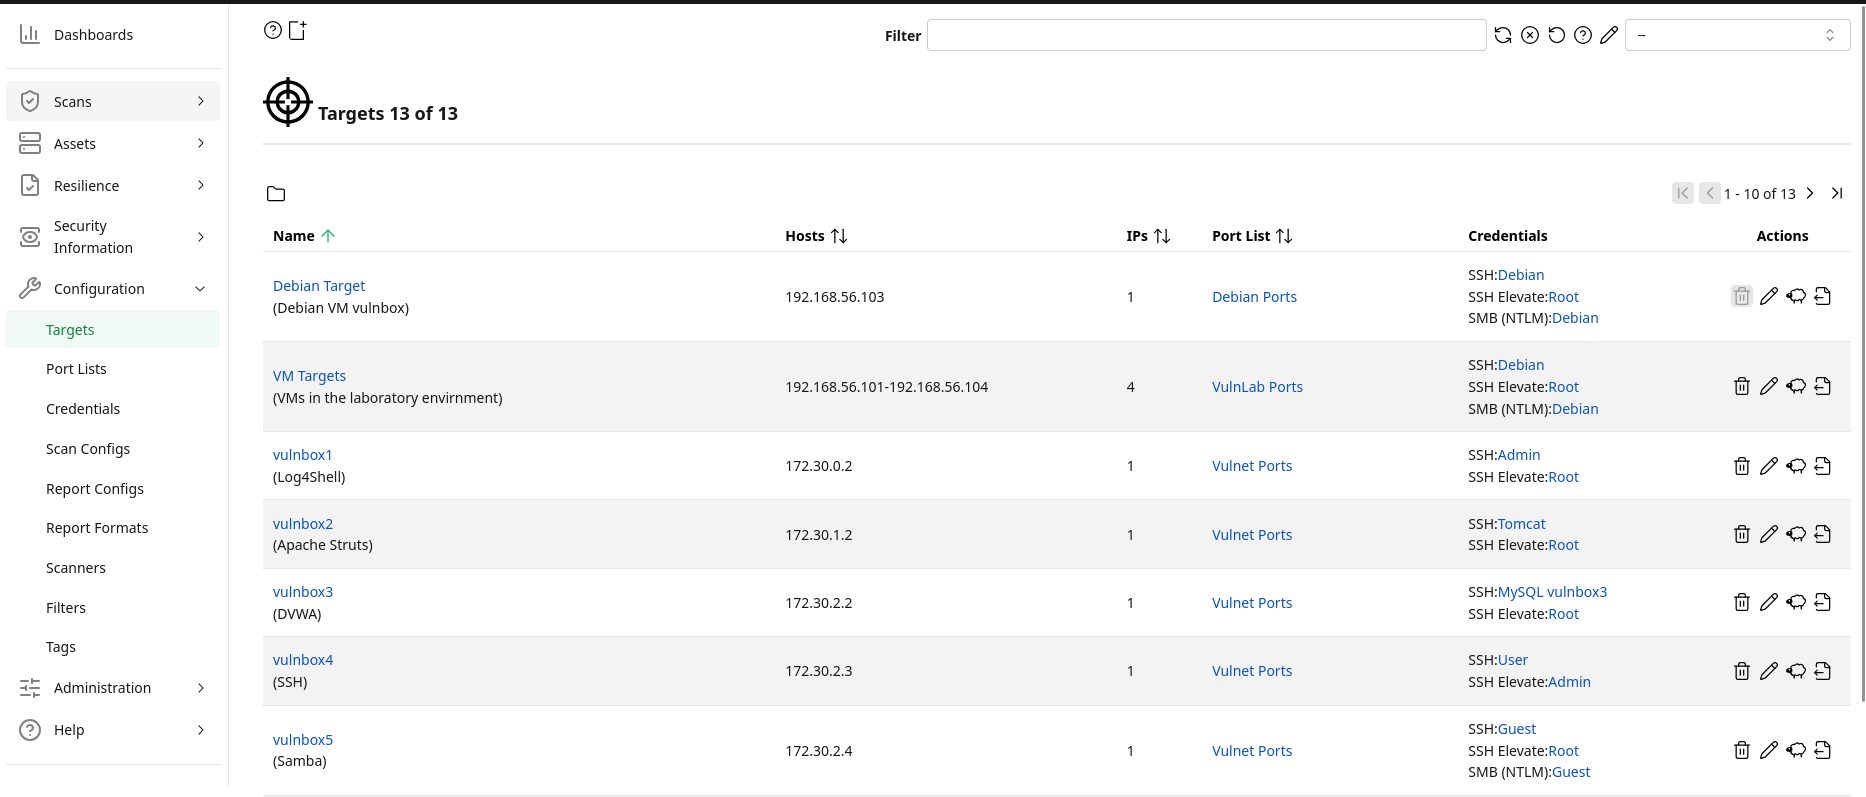
\includegraphics[width=0.9\textwidth]{images/openvas_conftargets.png}
	\end{center}

}

\frame{
	\frametitle{Target creation}
	\begin{columns}[T,onlytextwidth]
       \begin{column}{0.4\textwidth}
        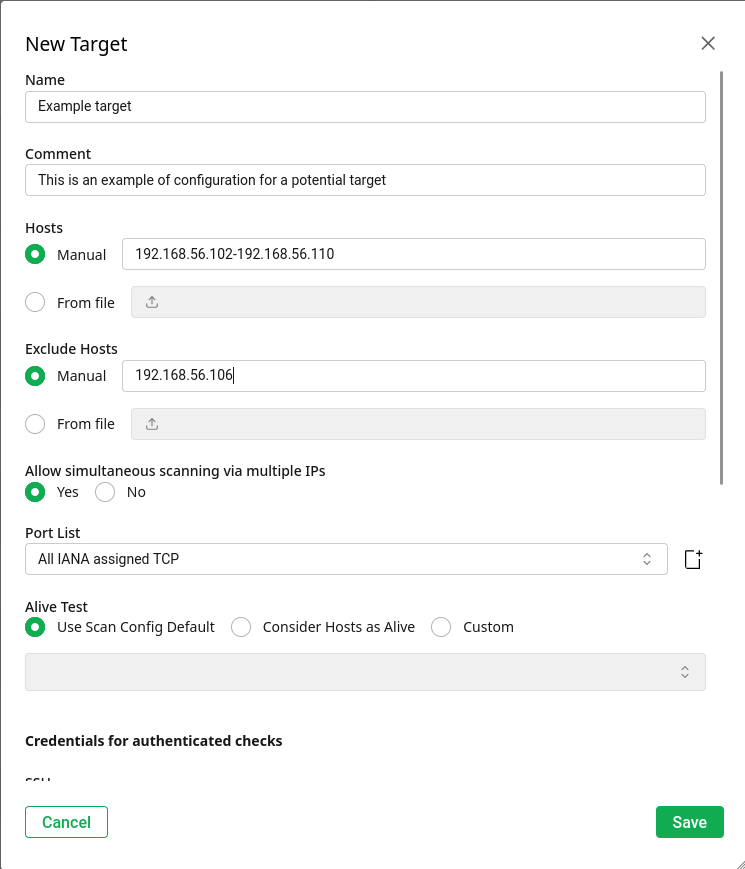
\includegraphics[width=\textwidth]{images/openvas_newtarget1.png}
       \end{column}
       \begin{column}{0.4\textwidth}
           \centering
           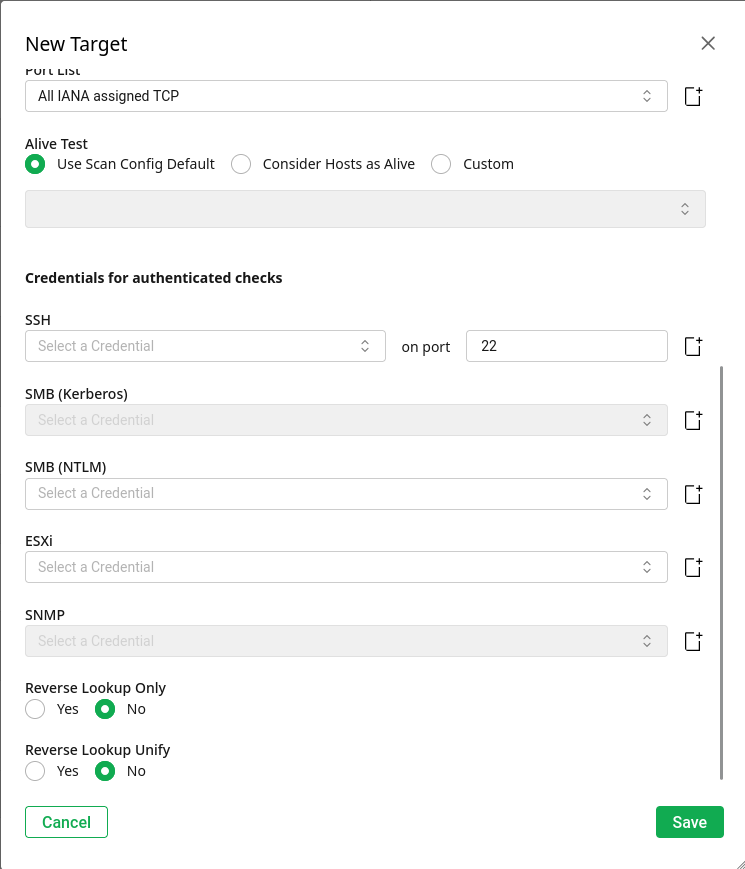
\includegraphics[width=\textwidth]{images/openvas_newtarget2.png}
       \end{column}
    \end{columns}
}

\frame{
	\frametitle{Scan configs}
	\begin{center}
		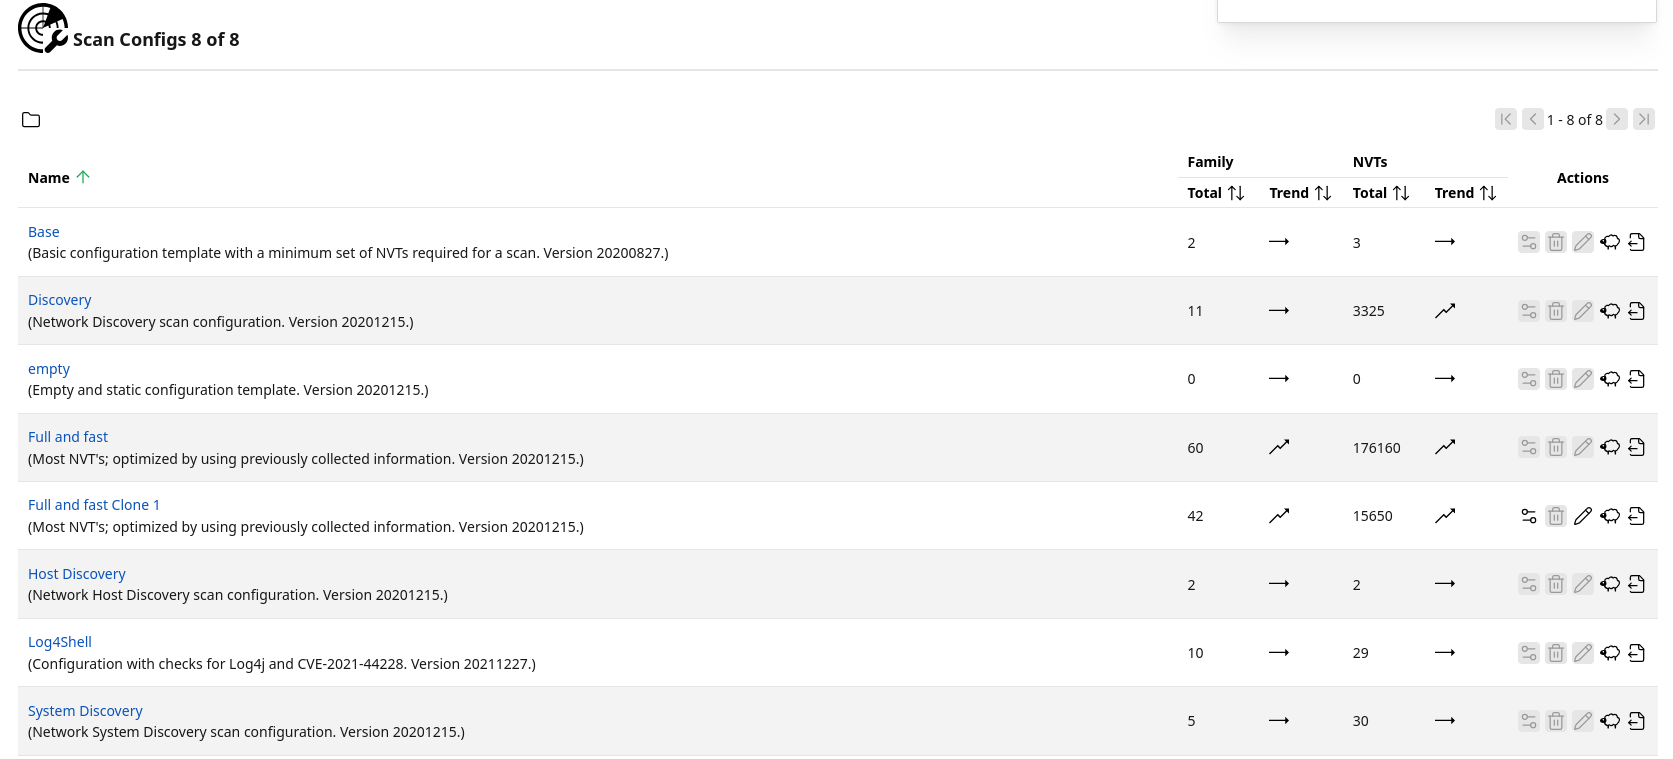
\includegraphics[width=0.9\textwidth]{images/openvas_scan_config1.png}
	\end{center}
}
\frame{
	\frametitle{Scan configs}
	% \begin{center}
	% 	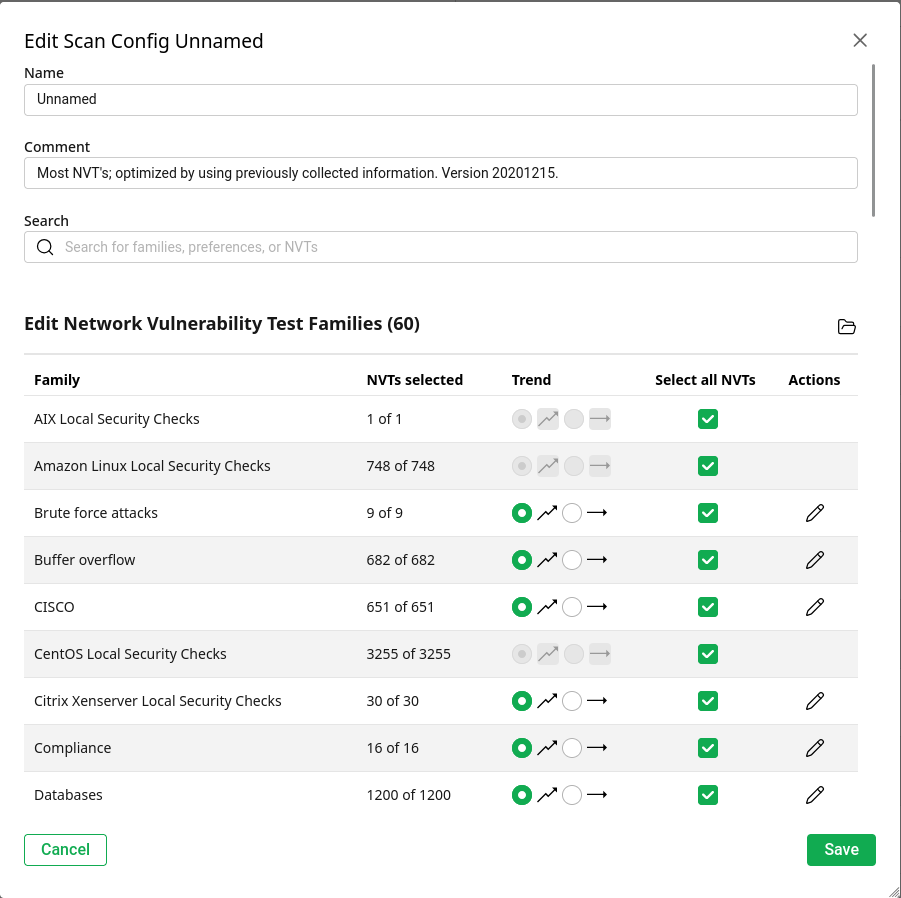
\includegraphics[width=0.5\textwidth]{images/openvas_scan_config2.png}
	% \end{center}

	\begin{columns}[T,onlytextwidth]
       \begin{column}{0.4\textwidth}
		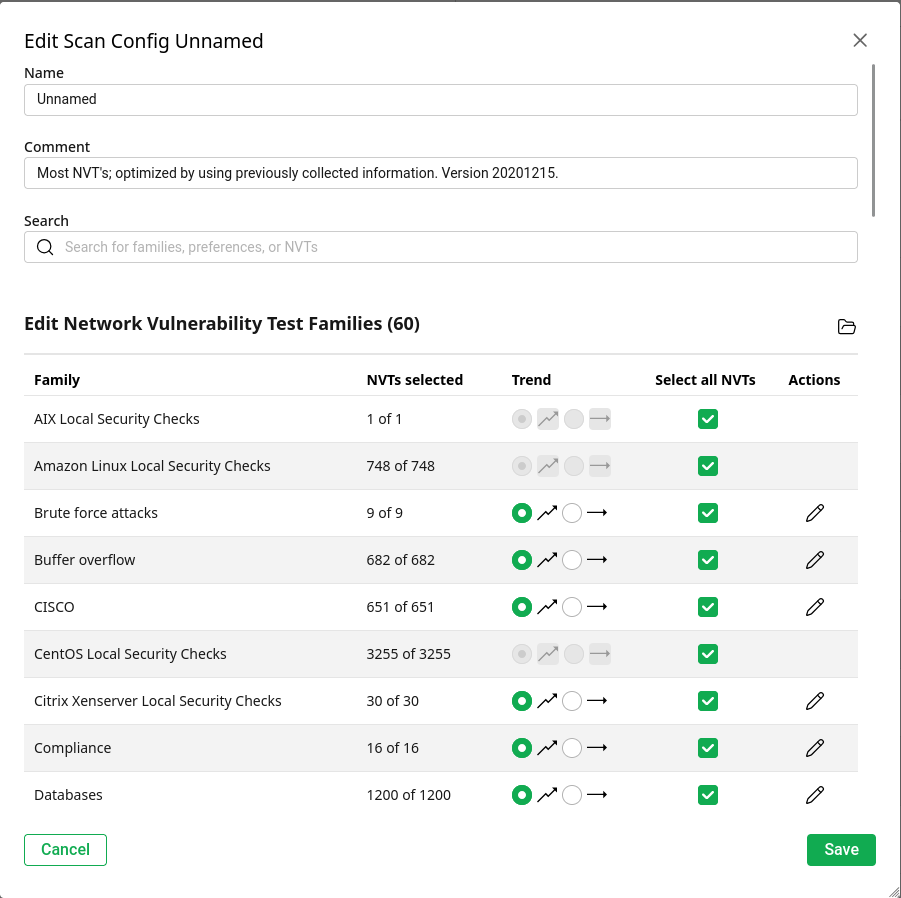
\includegraphics[width=\textwidth]{images/openvas_scan_config2.png}
       \end{column}
       \begin{column}{0.4\textwidth}
           \centering
		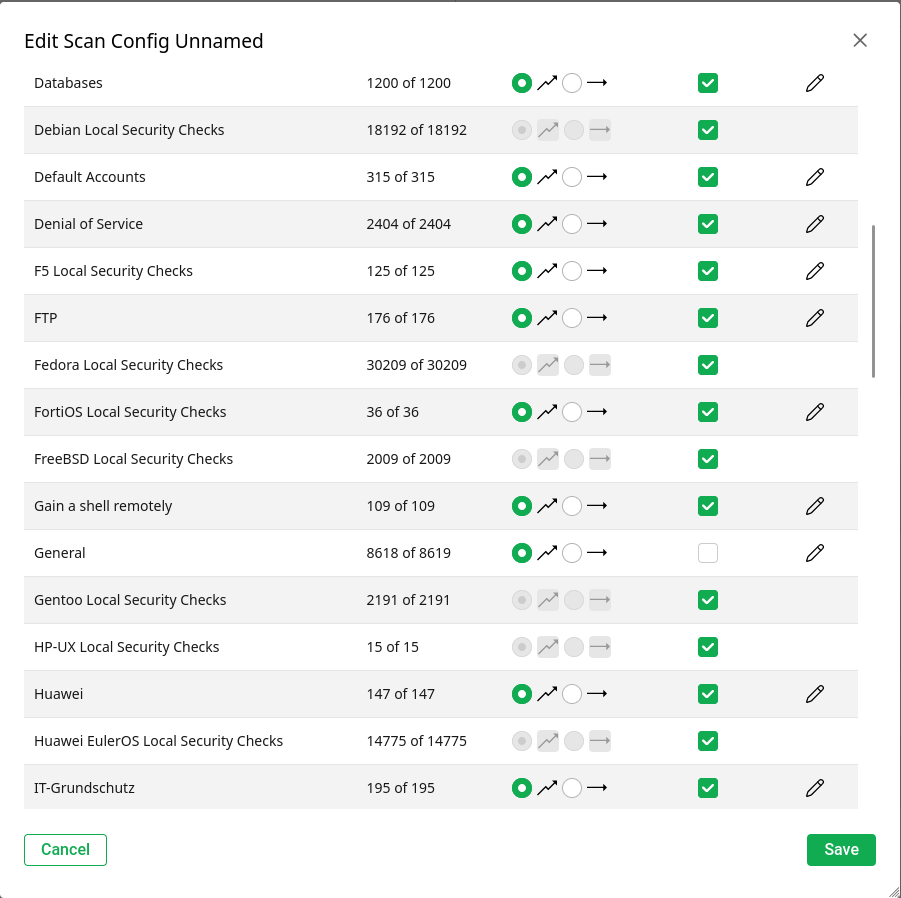
\includegraphics[width=\textwidth]{images/openvas_scan_config3.png}
       \end{column}
    \end{columns}
}
% \frame{
% 	\frametitle{Scan configs}
% 	\begin{center}
% 		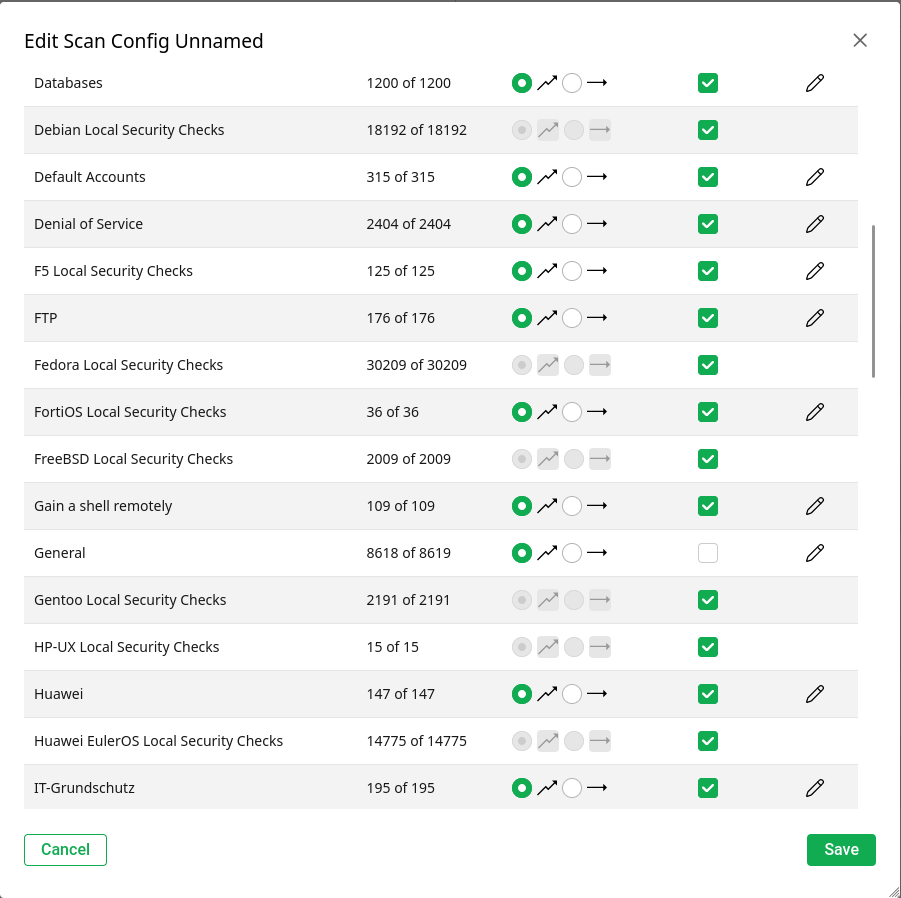
\includegraphics[width=0.5\textwidth]{images/openvas_scan_config3.png}
% 	\end{center}
% }

\frame{
	\frametitle{Scan interface}
	\begin{center}
		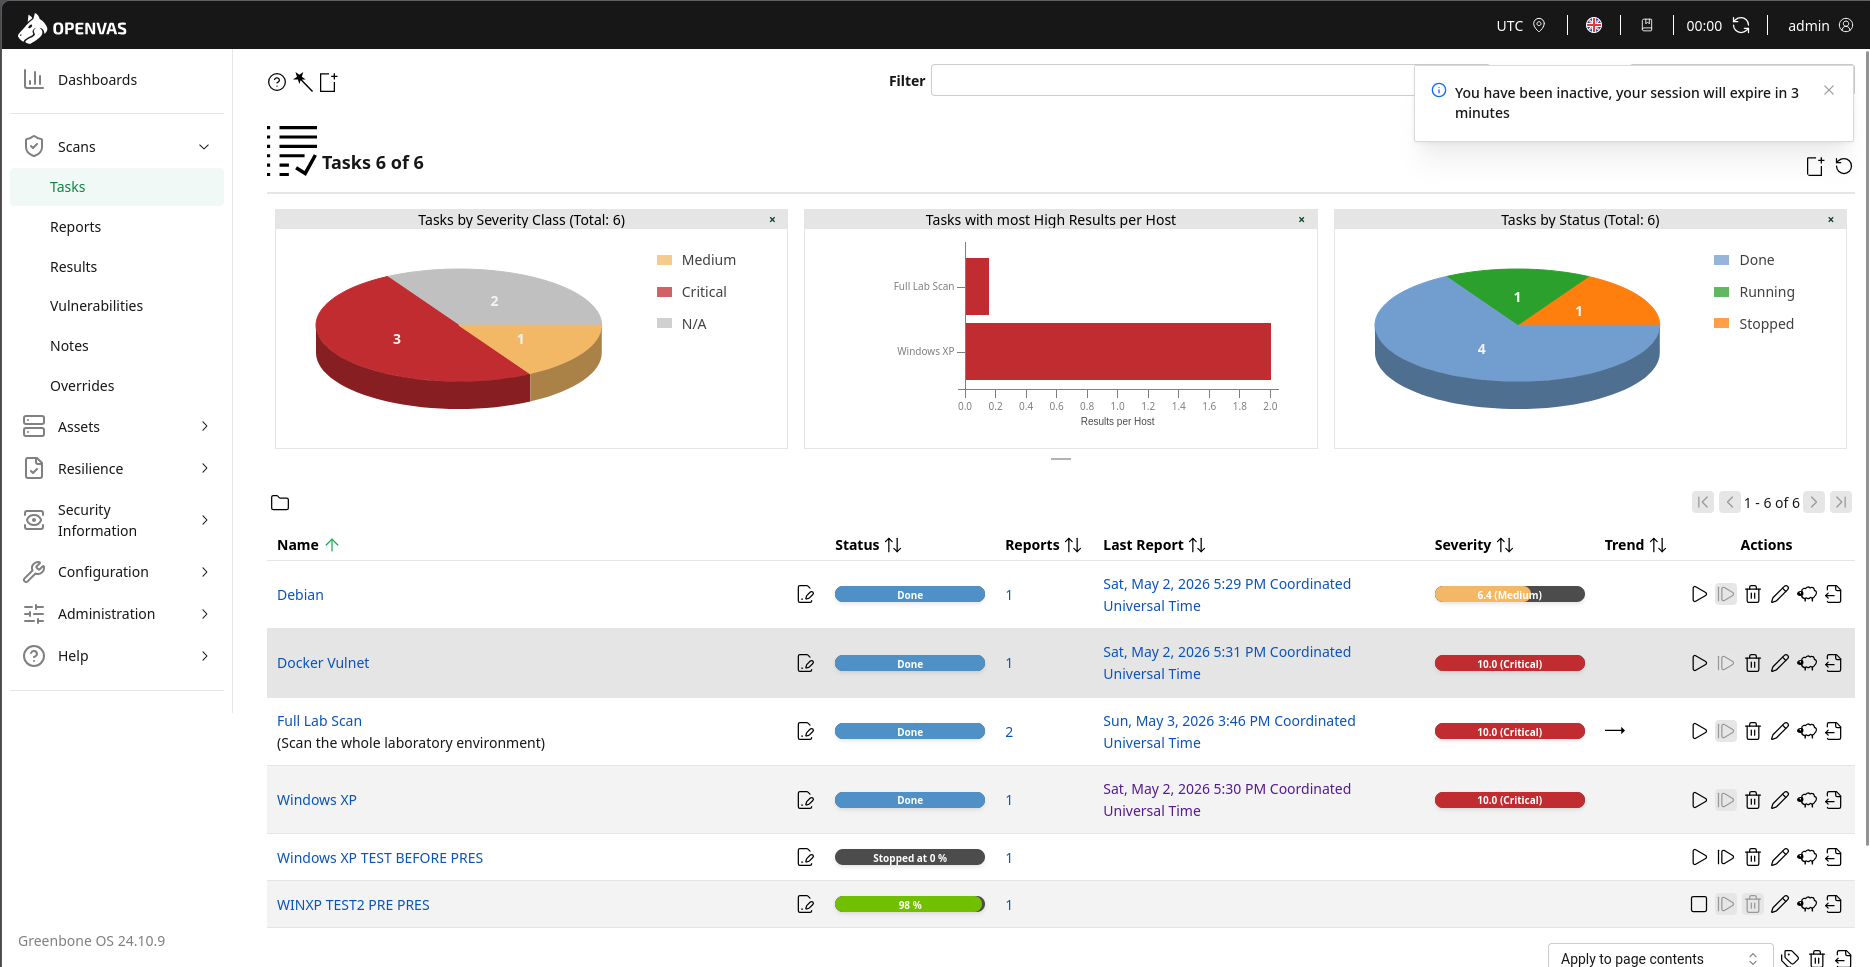
\includegraphics[width=0.9\textwidth]{images/openvas_scan_interface1.png}
	\end{center}

	%\begin{columns}[T,onlytextwidth]
    %    \begin{column}{0.4\textwidth}
    %        These are the 3 VMs:
    %        \begin{itemize}
    %            \item OPENVAS-FREE-24.10.9-VirtualBox
    %            \item Debian
    %            \item Windows XP
    %        \end{itemize}
    %        Configure the Network \underline{of all of them}
    %        by selecting the \textbf{Host-only Adapter} as network adapter 
    %        and choosing the network you created in the previous step.
    %    \end{column}
    %    \begin{column}{0.6\textwidth}
    %        \centering
    %        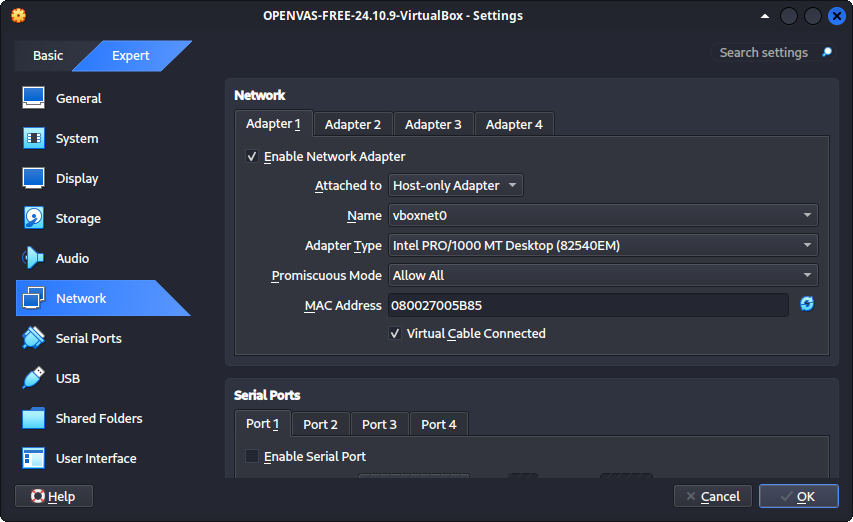
\includegraphics[width=\textwidth]{images/net_setup_3.png}
    %    \end{column}
    %\end{columns}
}

\frame{
	\frametitle{Task creation}
	\begin{columns}[T,onlytextwidth]
       \begin{column}{0.4\textwidth}
        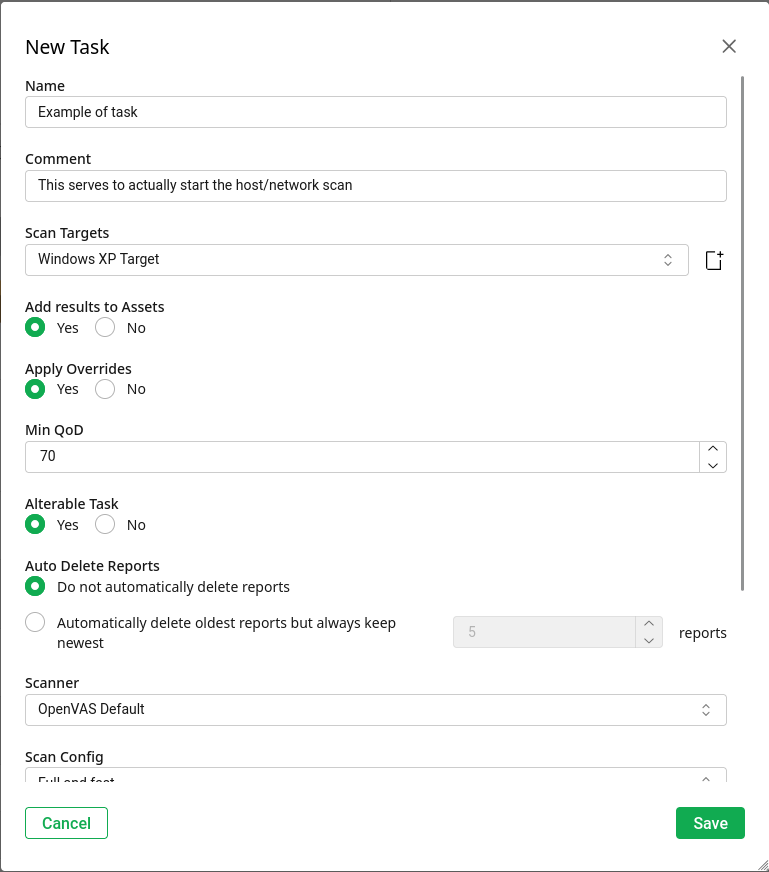
\includegraphics[width=\textwidth]{images/openvas_task_creation1.png}
       \end{column}
       \begin{column}{0.4\textwidth}
           \centering
           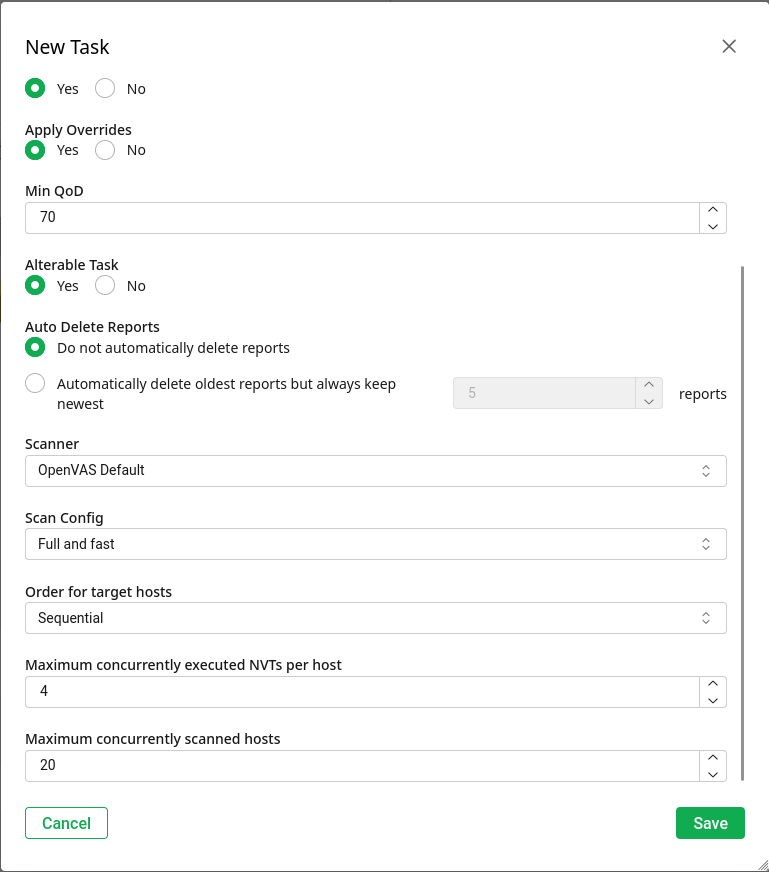
\includegraphics[width=\textwidth]{images/openvas_task_creation2.png}
       \end{column}
    \end{columns}
}





% \frame{
% 	\frametitle{Exercise: Scan for services on Windows XP}
% 	Try and start a scan for Windows XP on port 21 using Full and Fast preset
% 	\begin{itemize}
% 		\item Create the port record
% 		\item Create host record (should be 192.168.56.10x depending on the IP)
% 		\item Create a new task (remember to make it adjustable, otherwise you have to recreate it from scratch), remember to schedule it
% 	\end{itemize}

% }

\frame{
	\frametitle{Assets: Operating Systems}
	\begin{center}
		\includegraphics[width=0.9\textwidth]{images/openvas_asset_OS.png}
	\end{center}

}
\frame{
	\frametitle{Assets: TLS Certificates}
	\begin{center}
		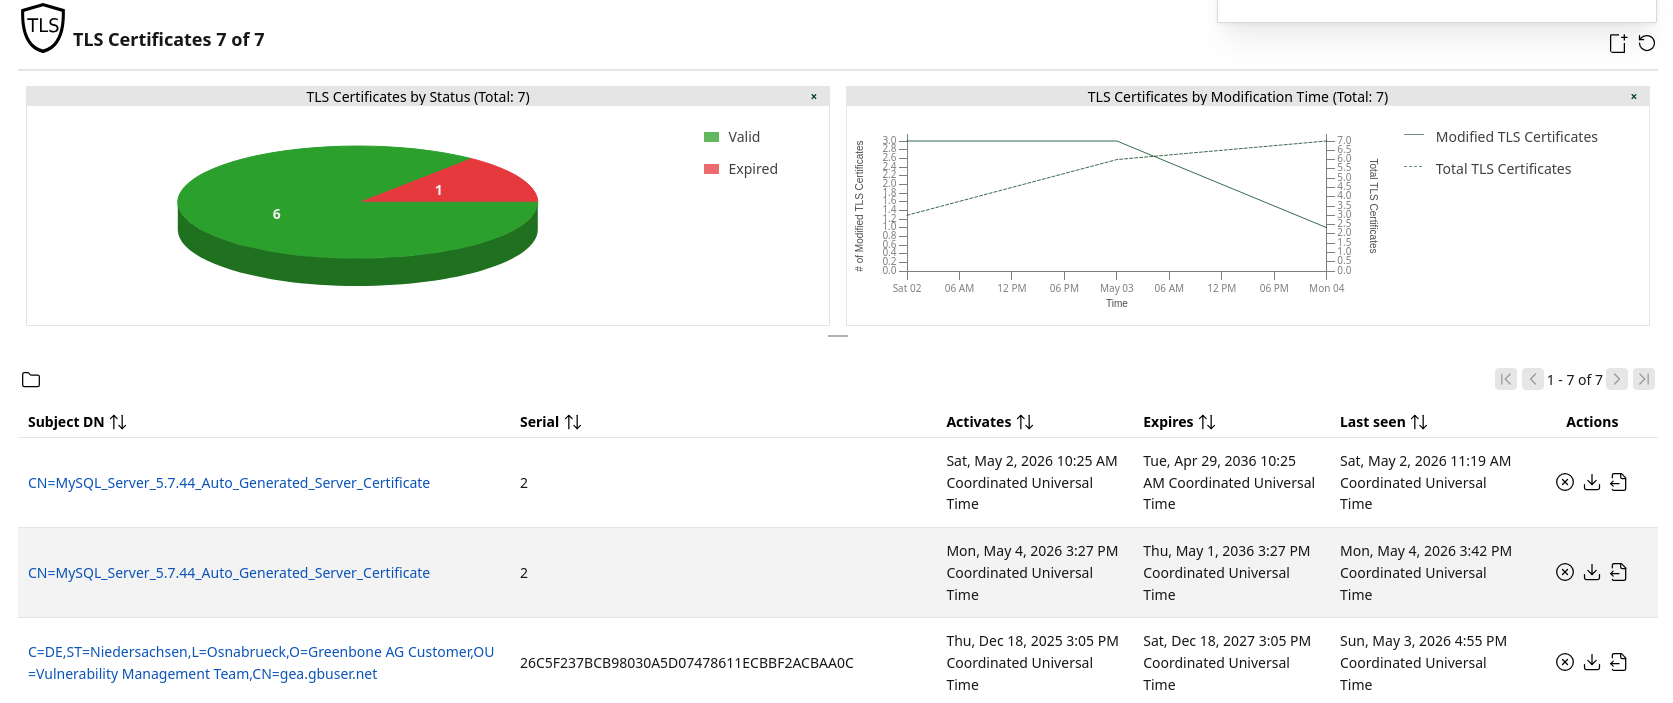
\includegraphics[width=0.9\textwidth]{images/openvas_asset_tls.png}
	\end{center}

}

\frame{
	\frametitle{Exercise: Scan for services on Windows XP}
	Try and start a scan for Windows XP on port 21 using Full and Fast preset
	\begin{itemize}
		\item Create the port record
		\item Create host record (should be 192.168.56.10x depending on the IP)
		\item Create a new task (remember to make it adjustable, otherwise you have to recreate it from scratch), remember to schedule it
	\end{itemize}

}



\frame{
	\frametitle{Reports}
	\begin{columns}[T,onlytextwidth]
		\begin{column}{0.3\textwidth}
		\begin{itemize}
			\item After a scan has been done, a report will be created citing everyting the tool founds.
			\item You can also see the severity of the Vulnerability he finds
		\end{itemize}
		\end{column}

       \begin{column}{0.6\textwidth}
           \centering
           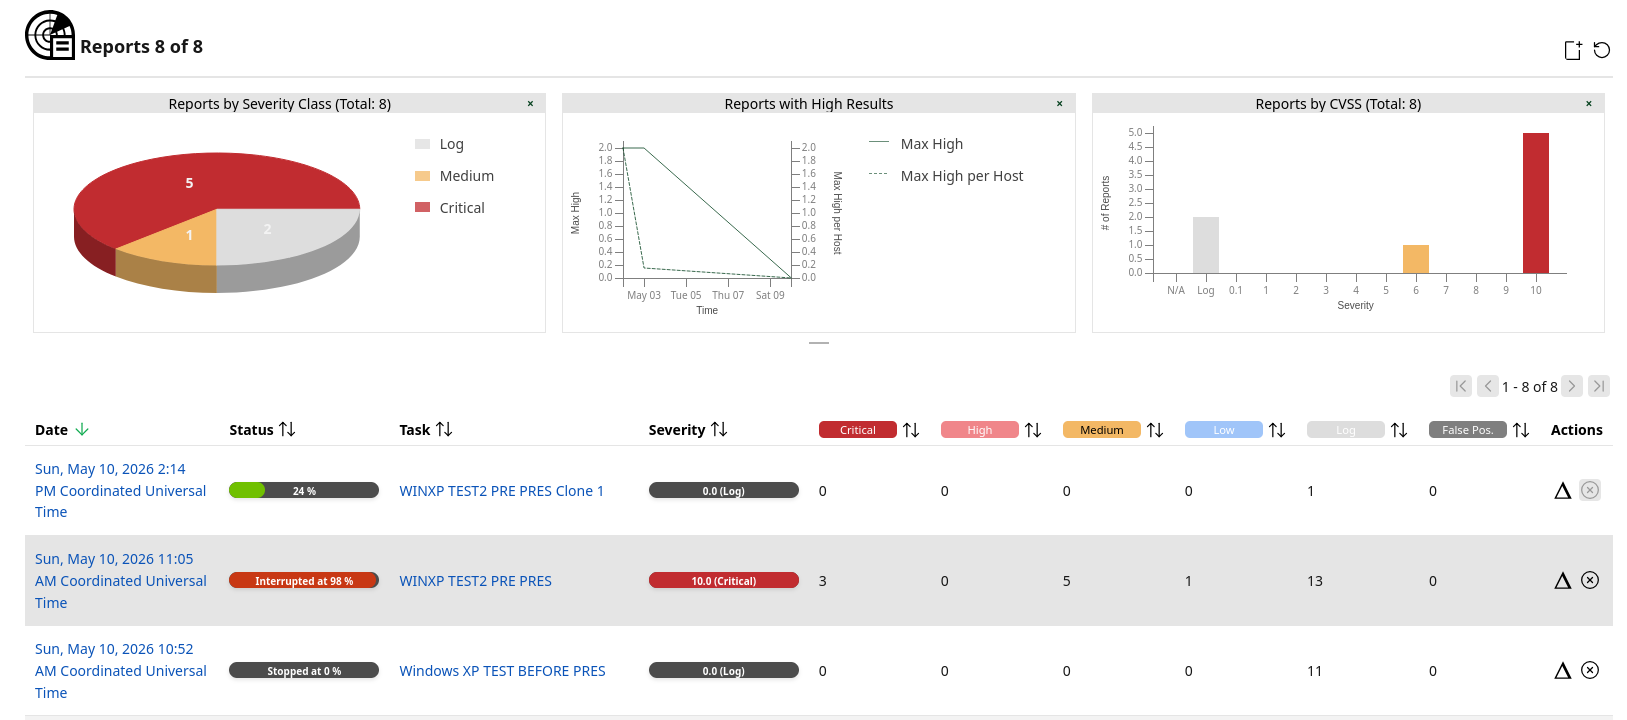
\includegraphics[width=\textwidth]{images/openvas_report.png}
       \end{column}
    \end{columns}
}

\frame{
	\frametitle{Results}
		\begin{columns}[T,onlytextwidth]
		\begin{column}{0.3\textwidth}
		\begin{itemize}
			\item Here you will see the results sorted by severity across all scans 
		\end{itemize}
		\end{column}

       \begin{column}{0.65\textwidth}
           \centering
           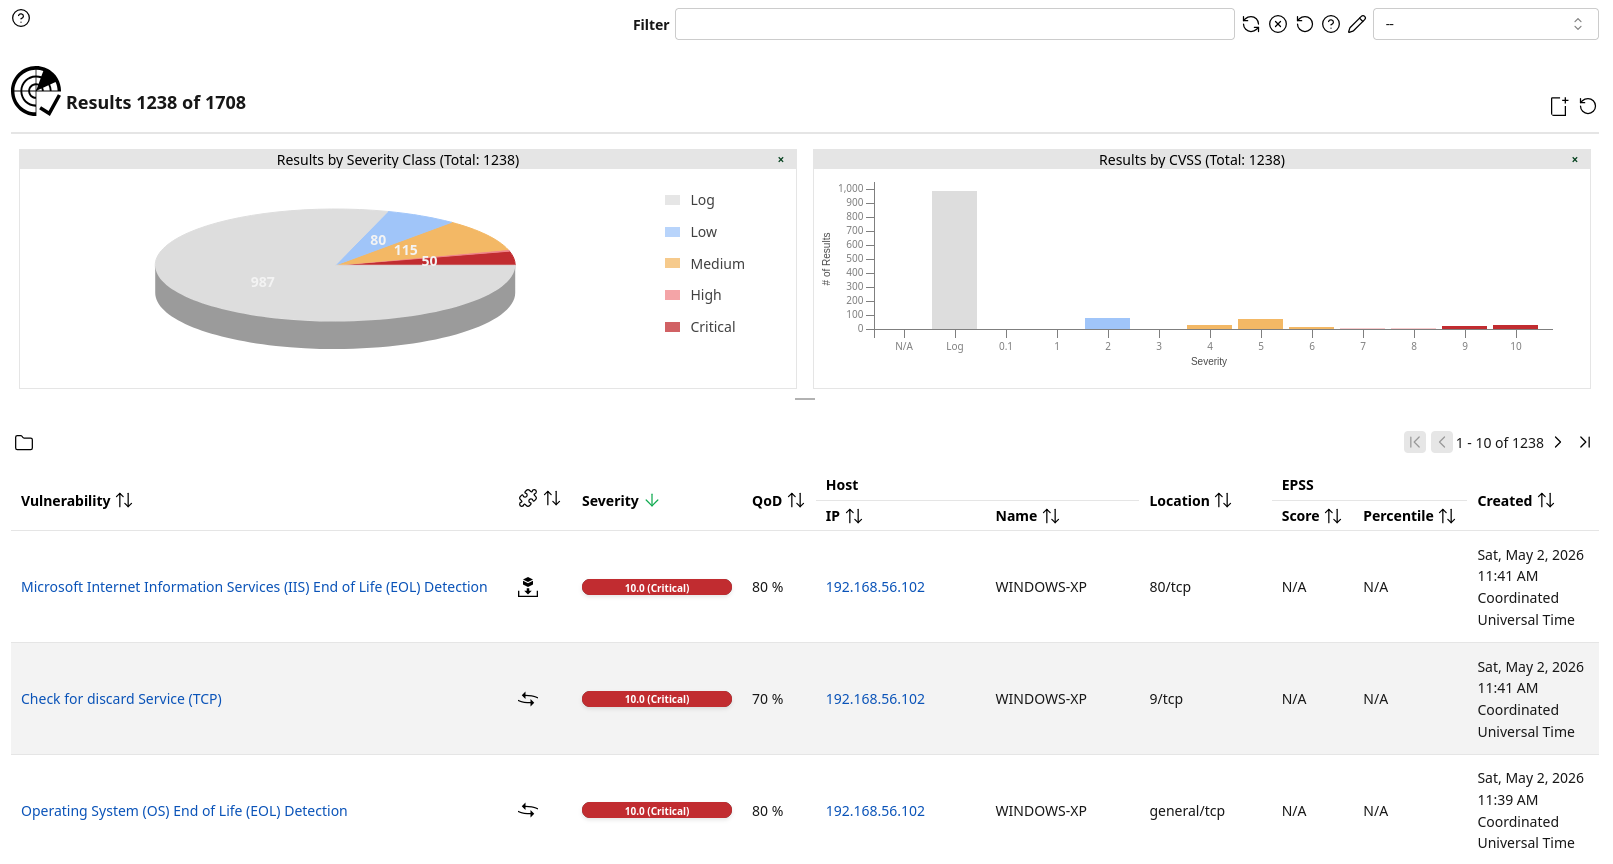
\includegraphics[width=\textwidth]{images/openvas_results.png}
       \end{column}
    \end{columns}
}


% TODO: Creare esercizio configuration scan configs e ripetere la scansione
% TODO: Spiegare differenze tra scan configs
% TODO: FIX ORDER
% contacts frame accepts main argument (will be in the centre left) and an optional argument (bottom)
% first line or two repeat the \author on the title page
% notice that language of the frame title is connected to the language of the logo
\contactsframe[We declare that we used Generative AI tools to improve grammar and clarity of the presentation.
No AI tool was used to design the structure of the presentation or generate crucial content.]
{\\
    Project repository avaiable at:\\

\includegraphics[height=0.6\baselineskip]{icons/white/github}\ \href{https://github.com/ozneroL541/network-security}{https://github.com/ozneroL541/network-security}\\
}

\end{document}

